\documentclass[a4paper,10pt]{article} % Artikel med 12pt text och A4 storlek.
%\documentclass[draft,10pt]{article} % Artikel med 12pt text och A4 storlek.
\usepackage[english]{babel} % Svensk avstavning istället för engelsk
%\usepackage[pdflatex]{graphicx}% De här två behövs för svenska
\usepackage[utf8]{inputenc} % UTF-8 encodad fil. Kan bytas ut mot latin1 om en vill...
\usepackage[T1]{fontenc}
\usepackage[authoryear]{natbib}
\usepackage{bibentry}
\usepackage{subcaption}
\usepackage{boldline} 
\usepackage{amsmath}
%\usepackage[allfiguresdraft]{draftfigure}
\usepackage{float}
\usepackage[margin=2.5cm]{geometry}
\usepackage{setspace}
\usepackage{color}
\usepackage{enumitem}   
\usepackage[T1]{tipa}
\usepackage{tabu}
\usepackage{textcomp}
\usepackage{rotating}
\usepackage{booktabs}
\renewcommand{\arraystretch}{1.3}
\usepackage{tabu}
\usepackage{longtable}
\usepackage{pbox}
\usepackage{setspace}
\usepackage{lscape}
%\usepackage{enumitem}
%\usepackage{enumerate}
\setcounter{secnumdepth}{4}
\setcounter{tocdepth}{5}
\usepackage{array}
\newcolumntype{?}{!{\vrule width 1pt}}
\newcolumntype{L}[1]{>{\raggedright\let\newline\\\arraybackslash\hspace{0pt}}m{#1}}
\newcolumntype{C}[1]{>{\centering\let\newline\\\arraybackslash\hspace{0pt}}m{#1}}
\newcolumntype{R}[1]{>{\raggedleft\let\newline\\\arraybackslash\hspace{0pt}}m{#1}}
%\usepackage{graphics}
\usepackage{graphicx}
\usepackage{subcaption}

\usepackage{lipsum}



\usepackage{footnote}
\usepackage{tipx}

\usepackage{wrapfig}
\usepackage[table,dvipsnames]{xcolor}
\usepackage{multirow}

\usepackage{titlesec}

\setcounter{secnumdepth}{4}


\usepackage{color}  
\usepackage{hyperref}
\hypersetup{
    colorlinks=true, %set true if you want colored links
    linktoc=all,     %set to all if you want both sections and subsections linked
    linkcolor=violet,  %choose some color if you want links to stand out
            urlcolor=blue,
            citecolor=Thistle,
}

\usepackage{xcolor}

\definecolor{hedvig_blue}{HTML}{7D81F5}
\definecolor{hedvig_lightgreen}{HTML}{81F093}
\definecolor{hedvig_darkgreen}{HTML}{0B8C1F}
\definecolor{hedvig_orange}{HTML}{FFB87A}
\definecolor{hedvig_red}{HTML}{FFD9E0}
\definecolor{hedvig_yellow}{HTML}{FCFFA8}



\setcitestyle{notesep={:},aysep={},aasep={\&}}
%\renewcommand{\labelitemi}{$\rightarrow$}
\usepackage{gb4e}

%\usepackage{draftwatermark}
%\SetWatermarkText{DRAFT}
%\SetWatermarkScale{4}

%\pagestyle{myheadings}

\noautomath
\title{Dissecting historical reconstruction: comparing computational approaches and the comparative method for Oceanic grammar}
%ste says: https://www.facebook.com/alan.elliott.125/posts/pfbid022H8vUKQxqKEE1e64DTcaJqXLDdruJEP8kpj5M89UtV6z8HHSTTTtYJVMVhZuBhsHl

\author{Hedvig Skirg{\aa}rd}
\setlength{\parindent}{0pt}
\setlength{\parskip}{1ex plus 0.5ex minus 0.2ex}

\begin{document}
\def\code#1{\texttt{#1}}

\thispagestyle{empty}
%\singlespacing

\maketitle
\thispagestyle{empty}

\tableofcontents
\newpage

%\textcolor{red}{This is a first draft based on the chapter text. I've modified it, and I'm in the process of modifying further. }



\begin{abstract}
Reconstruction is an essential part of historical linguistics. The traditional Comparative Method (CM) identifies regular sound correspondences and cognates and then infers states in proto-languages by three core principles: assume the fewest changes on the tree, assume plausible changes, and assume plausible combinations of features in proto-languages. However, there is no clear consensus on how to weigh the principles against each other, and many studies are not fully transparent regarding how precisely the principles are applied. This allows for subjective differences between studies which are hard to discern and replicate. This study aims to better understand the comparative method in general and Oceanic proto-language grammar in particular by comparing the reconstruction of structural features by classical historical linguists using CM to computational reconstructions with explicit and transparent mechanisms: Maximum Parsimony (MP) and Marginal Maximum Likelihood (ML). MP is similar to CM in that it infers the fewest amounts of changes along the tree. ML on the other hand infers rates of change based on the distribution of values and takes into account branch lengths. In addition, we explore an even simpler method of reconstruction, which ignores tree structure and takes into account only the most common feature in the daughter languages. The results indicate that all methods applied achieve a high level of concurrence with predictions from historical linguistics. 
% ste says: https://www.facebook.com/alan.elliott.125/posts/pfbid022H8vUKQxqKEE1e64DTcaJqXLDdruJEP8kpj5M89UtV6z8HHSTTTtYJVMVhZuBhsHl

%There are two possible
%This could indicate that historical linguists mainly make statements about the grammar of Oceanic proto-languages where they have a high amount of certainty, 

%The results show that CM produces reconstructions that are most similar to those generated by MP or MC. This suggests that, at least for this sample of languages and features, CM does not appear to take branch lengths into account. The methodological drawbacks of using MP and MC imply that we should possibly re-evaluate the way reconstruction is done in historical linguistics and take into account insights from new approaches, such as ML which makes sound assumptions which are likely to give better estimations of the state of proto-languages.


%Historical linguists use the comparative method to find sound correspondences, to reconstruct unattested forms and structures of proto-languages and to propose subgroups. Part of this process can be done computationally with new methods such as Maximal Likelihood. Such methods are more explicit in terms of the assumed underlying tree structure, data weighting etc. Studies in historical linguistics are not always as explicit. In this paper, we attempt to reconstruct the assumptions and implicit inner workings of the comparative method by comparing reconstructions made "by hand" by historical linguists to those derived from computational means. We also address areas of conflicts where different historical linguistics scholars disagree and evaluate what we can learn from computational methods regarding these issues. We estimate the grammatical structures of Oceanic languages in particular, using the Grambank dataset and trees published by Glottolog and \citet{grayetal_2009}. The results show that classical historical linguistics, for this dataset and trees, appears to mainly be an application of Maximum Parsimony, and we further discuss what this implies for the field of reconstruction of proto-languages. In the cases where historical linguists disagree, the results further shows that the most likely scenario is that proto-polynesian was ergative.
\end{abstract}
\newpage

\doublespacing
\section{Introduction}
\label{acr:intro}
Linguistic history offers us a unique and insightful window into our human past. By reconstructing the paths languages take, we can learn about our history and infer migration paths of people and cultures. By reconstructing the words and grammars of ancient languages, we can learn about communities long gone. Historical linguistics is devoted to this endeavour and has made great strides in our understanding of human history since its inception. The field has established methods which have enabled us to classify languages into language families and reconstruct words and grammars of proto-languages (unobserved ancestors of observed languages). Conclusions from historical linguistics are also impactful outside of linguistics, for example in archaeology and history studies. %ste says to insert ref

Linguists who work on historical reconstructions produce valuable and greatly inspiring work. However, one problem with the field is that analysis often relies on subjective evaluations of the evidence at hand and differing assumptions about what is plausible. This makes historical linguistics difficult to replicate. Historical linguists possess a great wealth of knowledge and understanding of a region and its cultures. All of this background knowledge underlying analytic decisions is not always made explicit and formally defined (possible due to lack of space and necessity). This makes the analysis difficult to evaluate for someone not as steeped in the literature and region.

In recent years, linguists have begun to apply computational phylogenetic methods from biology to the reconstruction of linguistic history. Biologists have, similarly to linguists, been interested in inferring trees of the genetic relationship between species, ancestral states and the tempo and mode of evolution \citep{atkinson2005curious}. Interestingly, the use of trees in linguistics and biology first occurred in publications just one year apart with \citet{schlegel1808sprache} publishing a tree of languages and \citet{lamarck1809philosophie} a tree of species.\footnote{However, as 
 \citet[370]{greenhill2015evolution} notes, it was not until Darwin's publication of \emph{The Origin of Species} in  \citeyear{darwin1859origin} that the concept of species trees in biology truly took off.} Biology and linguistics may have inspired each other, but methodologically the fields progressed separately for a long time \citep[370]{greenhill2015evolution}. Both fields are interested in answering similar questions: how are these languages/species related?, what was the earlier state of a language/species?, which traits are changing slowest? etc. The two fields have developed different methodologies, with biologists leaning more towards quantitative computational methods compared to linguists.
 
Historical linguistics is founded on the Comparative Method, which is a set of principles that can be applied to a set of languages and data to derive sub-groupings and ancestral states (see section \ref{sec:ars:metod:hist}). This approach has yielded great results, such as the inference of many language families and proto-languages, and has robust control for avoiding trivial similarities. However, one of the drawbacks of this approach is that it typically involves manual work and potentially subjective judgements. In contrast, computational phylogenetic methods are a set of tools that can be applied objectively in a systematic fashion. These approaches have the advantage of being able to be applied in exactly the same way across a large set of data and their mechanisms are very explicit. Computational approaches are not intended to replace traditional historical linguistics, but rather function as a complement effectivizing parts of the process. In this paper, we examine how often computational methods of reconstruction arrive at the same conclusions as traditional historical linguists using the Comparative Method. We will also investigate what the computational methods say when historical linguists disagree, and make new predictions about the grammar of proto-languages.

Applying computational methods of ancestral state reconstruction to linguistic data is becoming more common. \citet{jager2018using} apply three different methods (Maximum Parsimony, Maximum Likelihood and Minimal Lateral Networks) to cognate class reconstruction in three different language families. The aim of that study was primarily to evaluate how often the methods reconstructed the same state as what the authors label ``the Gold Standard'' (reconstructions by traditional historical linguists using the Comparative Method). The data that serves as input to the computational machinery was annotated by ``hand'' for cognacy by historical linguists, meaning that the identification of cognate classes is still a human affair --- it was the reconstruction itself given that information that was being evaluated. Their overall result was that Maximal Likelihood performed the ``best'', but that there were still several shortcomings. Most notable of these are the handling of horizontal transfer/reticulation, variation within languages and parallelled independent shifts. In this paper, we address horizontal transfer by using sets of trees from a Bayesian posterior, some of which may represent horizontal transfer history.

There are also two recent studies of Indo-European grammatical history: \citet{carling2021reconstructing} and \citet{goldstein_2022}. \citet{carling2021reconstructing} evaluate different theories of the history of morphosyntax of Indo-European by comparing to the product of computational Bayesian phylogenetic modelling. They find support for the ``canonical'' model of Indo-European syntax and illustrate clearly with case examples how their model works. Goldstein in his paper challenges a commonly applied principle in the reconstruction of Indo-European syntax; the ``frequency heuristic'' which holds that \emph{if the number of homologous elements (e.g., lexical cognates) in the daughter languages meets a minimum threshold (canonically three), their ancestor is reconstructed to the root of the tree}\citep[1/71]{goldstein_2022}. This is done because scholars argue that the true tree is unknown, and that this is an appropriate method in the absence of the true tree. Goldstein argues that the appropriate action is instead to carry out reconstruction on many different trees that represent possible histories, a Bayesian posterior tree sample. He argues that this is methodologically more sound and the results of his approach are in accord with the consensus in historical linguistics, thus strengthening their validity.

Both \citet{carling2021reconstructing} and \citet{goldstein_2022} use a Bayesian method of ancestral state known as Continuous-Time Markov Chain (CTMC)\footnote{The main difference between the methods of \citet{carling2021reconstructing} and \citet{chang2015ancestry} is that \citet{carling2021reconstructing} use a tree structure informed by \citet{chang2015ancestry} and comparative-historical \emph{communis opinio} and vary the branch lengths 10,0000 times in a principled and informed manner to generate 10,000 different trees while \citet{goldstein_2022} takes 100 random samples directly from the posterior of \citet{chang2015ancestry}.}. This approach comes with certain important assumptions, to quote from \citet[77]{goldstein_2022}:

\begin{quotation} \emph{
CTMCs model language change as a stochastic phenomenon with rate parameters that govern the amount of time between transition events. It is worth highlighting the assumptions that these models bring with them. First, character states at the nodes of a tree are assumed to depend only on the state of their immediate ancestors and the length of the branch along which they evolved (Cathcart 2018:4). Second, the probability of a transition depends only on the current state of a language. Its previous history is irrelevant. This is known as the markov property. Finally, rates of gain and loss are assumed not to vary across the tree.}
\end{quotation}

For more details on the methods, please see  \citet{goldstein_2022}, \citet{pagel2004bayesian}, \citet{ronquist2004bayesian} and \citet{liggett2010continuous}. This method is not identical to, but relatively similar to Stochastic Character Mapping \citep{huelsenbeck2003stochastic}.

Computational approaches to reconstruction not only allow us to effectivize the process by inferring the prior states of hundreds of traits in a short span of time, but it also allows us to apply exactly the same principles in exactly the same way to all pieces of data. This is much harder to do manually, since different scholars may use slightly different assumptions and judgement when applying the traditional Comparative Method. 

The particular study object of this paper is the Oceanic language subgroup of the Austronesian family and the grammatical features of four of its proto-languages. We use information about the extant daughter languages from the Grambank dataset \citep{grambankwebsite} to infer the structure of proto-languages. The computational methods are applied using two published trees of Oceanic: Glottolog 4.0 and \citet{grayetal_2009}. Findings from the historical linguistics literature have been translated into data-points in the Grambank format for four specific proto-languages: Proto-Oceanic, Proto-Central Pacific, Proto-Polynesian and Proto-Eastern Polynesian. The computational methods take as input the language-level data points in the Oceanic subgroups and then infer grammatical states of proto-languages in the tree. The state of the aforementioned four proto-languages are extracted for each tree and method and compared to conclusions from classical historical linguistics. The results are evaluated in terms of concordance between each method and the predictions from classical historical linguistics. We are evaluating how much they agree, not necessarily which one is correct. Which method is correct should be estimated based on the conceptual underpinnings and assumptions of the method and how plausible that model of change is. From the exercise in this study we can learn about which method agrees most with classical historical linguistics, and therefore dissect the comparative method into explicitly formally objectively defined mechanisms.

There is one area of Oceanic grammatical reconstruction where there is considerable disagreement. This concerns the nature of the alignment system of Proto-Polynesian and Proto-Central Pacific. These issues will be investigated and evaluated separately from the overall results of how much agreement there is between classical historical linguistics and the computational approaches.

Finally, this study also yields predictions about grammatical features of the four proto-languages that were not addressed by the historical linguistics studies surveyed here.

%The tools of computational reconstructions are different from classical historical linguistics, and the data used in this chapter, the Grambank dataset, is different from the source material that historical linguists work with. This is further discussed in section \ref{sec:ars:metod:hist}


\section{Background}
\label{recon_grammar}

\subsection{The methods of traditional historical linguistics: the Comparative Method}
\label{sec:ars:metod:hist}
In order to interpret the differences between the results of the computational approach versus the classical historical linguistics approach, it is first necessary to clarify the different methodologies and the consequences of them for the study at hand. This section lays out the fundamental principles of historical linguistics and how they relate to this paper.

The core method by which historical linguists reconstruct language history is known as the ``Comparative Method''. The Comparative Method is based on finding words or morphemes in different languages that have the same (or similar enough) meaning and that display non-trivial systematic phonological similarities. By investigating these sets of words, it is possible to deduce which are inherited from a common shared ancestor, i.e. are cognates. For example, \citet{blust2004}, \citet{greenhill2011pollex} and many others have reconstructed that M\={a}ori /toru/ (meaning `three') derives from the same word in an ancestral language as Hawai'ian /kolu/ (`three') does. These two words are ``cognates'' of each other and this information can be used to reconstruct a form for proto-Polynesian. Furthermore, many words that mean the same/similar thing in M\={a}ori and Hawai'ian show this pattern of t/k, e.g. M\={a}ori: /mate/, Hawai'ian: /make/ `to be dead'  and M\={a}ori: /whitu/, Hawai'ian: /hiku/ `seven' \citep{ABVD}. There is a systematic correspondence between these two sounds; regularly when there is a /t/ in M\={a}ori there is a /k/ in the corresponding position in Hawai'ian. This is known as a \emph{systematic sound correspondence}. Further research into more languages of this family shows that Hawai'ian /k/ is more likely to be an innovation and M\={a}ori /t/ a retention from an older proto-language (c.f. in the Austronesian language Amis of Taiwan `three' is /tulu/). Therefore, we can reconstruct that the change went from /t/ $\rightarrow$ /k/.

% \citep{ABVD})\footnote{Note that there are two /k/ sounds in Oceanic languages. One stems from Proto-Oceanic *t and the other from POC *k. See more details in \citet{blust2004}.}. 

Historical linguists use cognates and systematic sound correspondences to develop hypotheses about forms in unobserved proto-languages and to propose sub-groupings based on shared innovations (c.f. how biological cladistics finds relationships between species based on shared derived characteristics from common ancestors \citep[16-17]{maclaurin2008biodiversity}). The Comparative Method provides us with a) sets of words which derive from the same word in an ancestor language (cognates), b) sequences of sound changes from proto-languages to the current observable daughter languages and c) a tree or network structure of the relationships between languages. 
 
The processes of subgrouping and reconstruction are done in tandem in historical linguistics; they are estimated simultaneously. Subgroups are proposed based on shared innovations. In order to determine what is and what is not an innovation, a certain amount of reconstruction is necessary. In order to make reconstructions, some of the tree structure needs to be approximated. Pawley (personal correspondence) notes that most of the subgrouping done in historical linguistics tends to be at the lower level. In this paper, we are only focussing on the reconstruction --- not on the identification of regular sound correspondences, cognates or subgroups.
 
The Comparative Method in historical linguistics relies on knowledge of probability of phonological shifts (/s/ is more likely to become /h/ than it is to become a /k/\footnote{Historical linguists do concede that there are instances of irregular sound change \citep{blust1996neogrammarian, campbell1996sound} and that while they can often be explained by contact, analogy or avoidance of homophony, they sometimes remain unexplained.}) and on probable semantic shifts. In the above example from M\={a}ori and Hawai'ian, the words /toru/ and /kolu/ both mean `three', but it is possible for cognates to have less similar meanings. For example, \citet{pawley2005meaning} reconstructs the proto-form *\emph{panua} as meaning `land' or `inhabited territory'. In daughter languages, this has changed to `place', `community', `village', `house', `people', `world' and `weather'. These are related meanings, but not identical. Historical linguists aim to have plausible semantic connections between words that are proposed to stem from the same proto-form, they cannot be too dissimilar.

%list the reconstruction */gaawari/ for Proto-Polynesian as meaning `weak, feeble'. In some of the daughter languages, words deriving from this Proto-word are listed as meaning `bent', `weak', `soft' and `slack (of man)'. These meanings are judged to be plausible semantic extensions of the proto-meaning such that they can be said to be related ---- to be cognates. 

%\footnote{In order to estimate what semantic shifts are reasonable, linguists can study colexifications in contemporary languages. These are instances of different meanings that are expressed by the same word. In the Database of Cross-Linguistic Colexifications (CLICS), users can explore clusters of colexifications, for example: the concept ``sun'' is more closely linked to ``day (not night)'' than it is linked to ``name'' ) \cite{list2018clics2}.}

The Comparative Method is typically applied to sound changes and words, but it can also be applied to structural features. \citet[17-22]{clark1976aspects} wrote about Proto-Polynesian syntax for example. He outlines three important principles for reconstruction that are relevant to words, sounds and grammar:

\begin{enumerate}[label=(\roman*)]
\item the number of changes posited
\item the plausibility of the changes posited
\item the plausibility of the reconstructed language as a human language (i.e. the degree to which the reconstructed traits work well in harmony with each other)
\end{enumerate}

The first of these principles is the same as what is known in phylogenetics as ``Maximum Parsimony''. The idea is to reconstruct states in proto-languages such that there are as few changes as possible between nodes in the entire tree. \citet[17-22]{clark1976aspects} explains how this works by positing an example of seven languages where there is a majority of one feature, X, and fewer of another, Y. Fig.~\ref{fig:clark_tree} illustrates this example. If we only examine which feature is the most common, we should reconstruct X at the root of this tree. However, this would result in 2 changes (one each between the root and tips A and B). If we instead reconstruct Y at the root, we would only need one change (between the root and PC-G). The solution where we reconstruct Y at the root results in fewer changes --- it is the most parsimonious.
 
\begin{figure}[h]
\centering
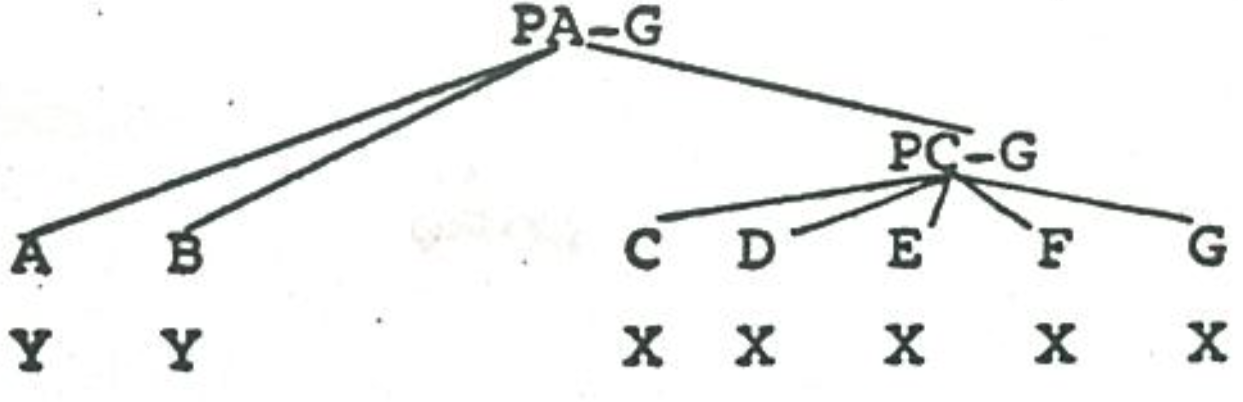
\includegraphics[width=8cm]{illustrations/Clark_1977_tree.png}
\caption{{Tree from \citet[19]{clark1976aspects} illustrating Maximum Parsimony.}}
\label{fig:clark_tree}
\end{figure}

It is important to note that Maximum Parsimony does not take into account the length of branches, only the changes between each node of the tree (regardless of how far apart they are). Furthermore, Maximum Parsimony makes the implicit assumption that the slowest rate of change is the accurate one. This is unlike Maximum Likelihood which does take into account branch lengths and allows rates of changes to be dynamically estimated (more on this in section \ref{sec:asr_methods}).

%The plausibility of the reconstruction language to be a human language relies on knowledge about which traits are likely to go together, and which would represent a combination that is veyr implausible. For example, if a language has a dual number category for nouns, i.e. signalling that the number of items is 2, it is likely to also have general plural number. If a reconstruction produces a language with a dual but not a plural, this is cause for concern as this is very unlikely according to linguists. The same is true of the plausibility of the changes from state to state themselves, some changes are assumed to be more frequent and common than others. However, linguists rarely spell out all of these assumptions explicitly in historical reconstruction, which makes it hard to evaluate what is happening. It also makes it difficult to incorporate these concepts in computational reconstruction. 

%Integral to the reconstruction of forms in historical linguistics is \textbf{Maximum Parsimony}. Maximum Parsimony is a method of reconstruction ancestral states (in this case grammatical features of proto-languages) in such a way that there is as few changes as possible from the root to every tip (language). 


\subsubsection{Disagreements in historical linguistics}
Reconstruction in historical linguistics includes judgements of plausibility. This requires some assumptions about what are plausible features to co-occur in language, and which pathways of language change are more plausible than others. For example, it is rare to find a language that has a gender distinction in first person, but not in third (though not impossible; c.f. \citet{wals-44}). If the most parsimonious reconstruction results in a proto-language with many rare features or unusual combinations of features, it may require reconsideration. If something is rare in the languages that exist today, we would expect it to be rare also in past languages. Similarly, changes from certain states to others are assumed to be less plausible. For example, a language going from having no marked dual number on nouns to having trial number would be taken as unusual by most linguists \citep[c.f.][8]{kikusawa_2006_pro_number}. 

Plausibility is important in reconstruction, both in linguistics and in biology. However, this principle is sensitive to differing assumptions and theories. What is more plausible as a reconstructed language or species may differ from scholar to scholar. Besides debates over precise sub-groupings, many arguments in historical linguistics boil down to disagreements about plausibility. This is also true of the different reconstructions of the alignment system of Proto-Polynesian.

\citet{clark1976aspects} disagrees with \citet{hale_1968}, \citet{hohepa_1969}, and \citet{chung1978} on the state of Proto-Polynesian syntax on these grounds. Chung, Hale and Hohepa argue for a theory that is technically less parsimonious, but which they say is more plausible. They posit that Proto-Polynesian had a nominative-accusative case marking system\footnote{Hale, Hohepa and Chung actually suggest three different specific theories for this reconstruction. For a summary of the differences between the proposals, see \citet[247-249]{chung1978}.}. If this was the case, that would mean positing more changes along the tree than if we assumed, as \citet{clark1976aspects} does, that the Proto-Polynesian language was ergative-absolutive. This is due to S\={a}moan and Tongan both having ergative-absolutive marking and both splitting off early (in most accounts of the Polynesian tree) from Proto-Polynesian compared to the rest of the group which most often lacks ergative-absolutive marking. Fig. \ref{poly_GB409_tree} shows the Polynesian tree with Grambank feature GB409 values marked out\footnote{Grambank feature GB409 asks if \emph{any} ergative flagging is present. In some instances, the system is not wholly or primarily ergative, but ergative marking is present. It is possible that the scholars involved in the debate would not classify such languages as ``ergative-absolute'' languages.}.

\begin{figure}[H]
\centering
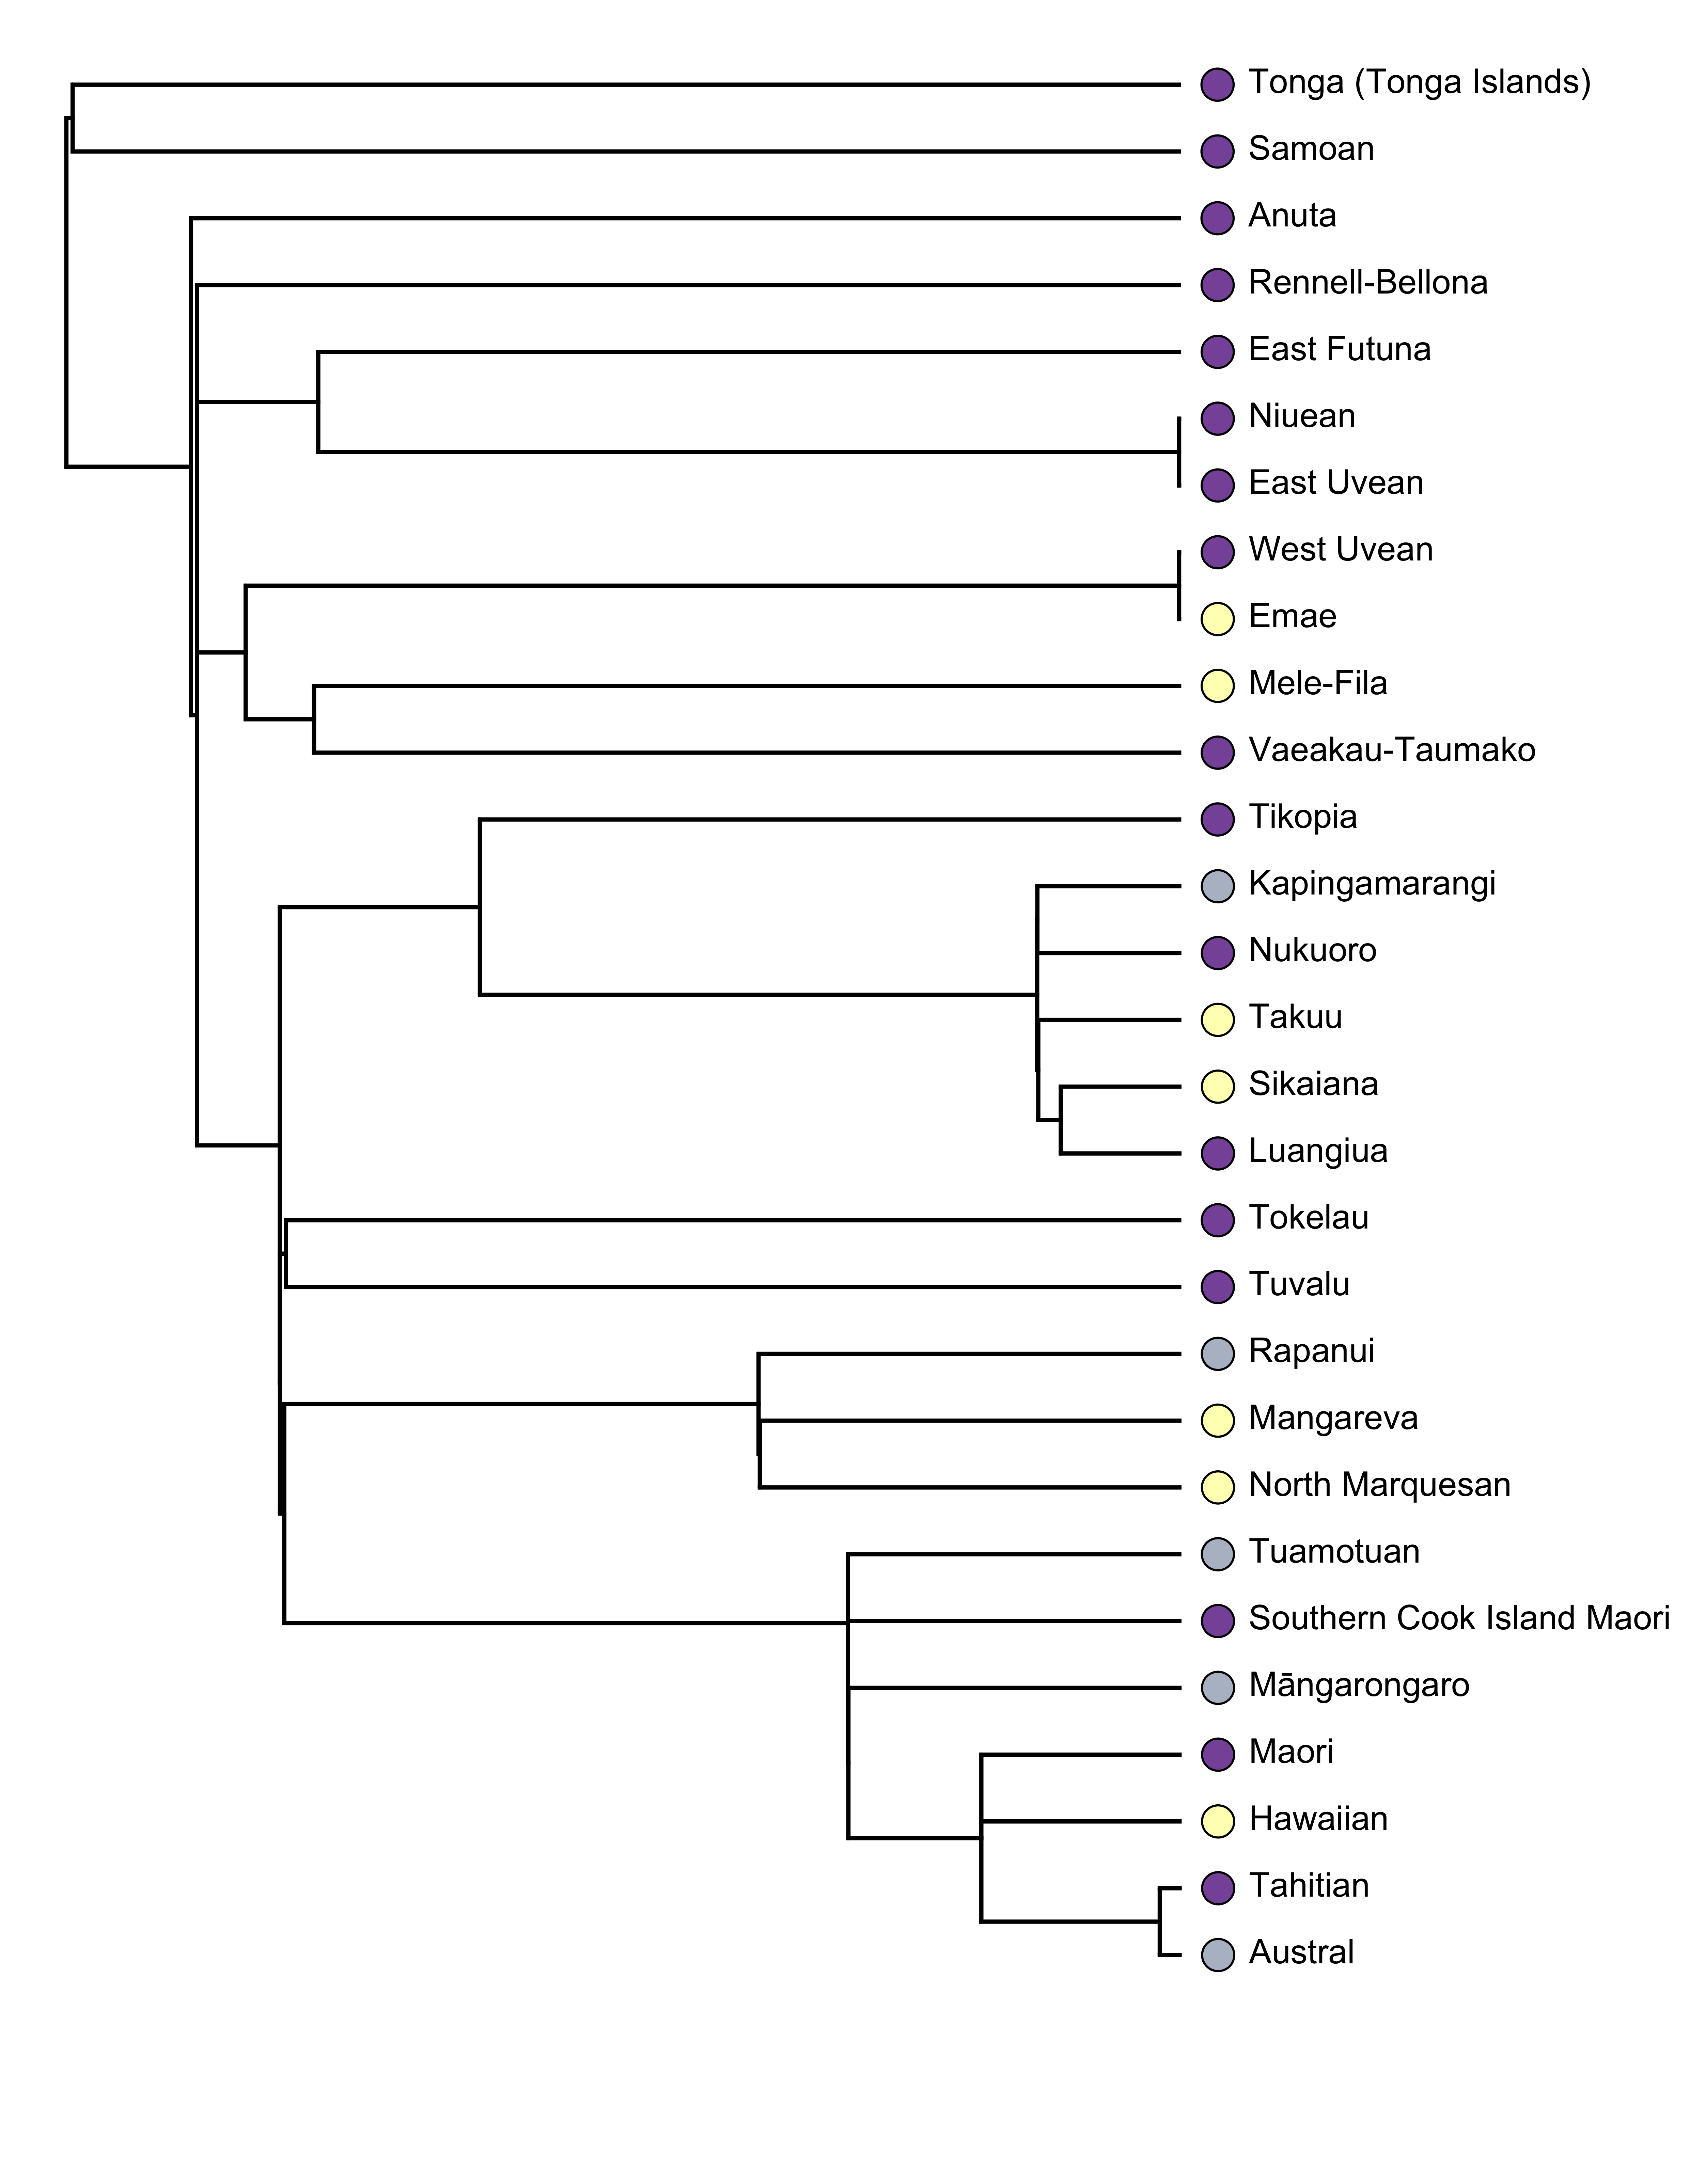
\includegraphics[width=9cm]{illustrations/plots_from_R//tree_plots/poly_tree_example.png}
\caption{{The Polynesian languages in the \citet{grayetal_2009} Maximum Clade Credibility Tree-tree, with the coding of Grambank feature GB409 ``Is there any ergative alignment of flagging?'' marked out. Purple = Yes, Yellow = No and white = Not enough information/not clear.}}
\label{poly_GB409_tree}
\end{figure} 

Chung's critique of Clark's proposal is three-fold: 
\begin{enumerate}[label=(\alph*)]
\item the tree used is not an accurate representation of the language history (there was more interaction between S\={a}moan and Tongan after splitting, i.e. horizontal transfer)
\item it is possible that the Proto-language contained variation and was undergoing change that was only fully realised in some of the daughters
\item the morpho-syntactical historical process itself is less plausible
\end{enumerate}

In a review of \citet{clark1976aspects}, Chung writes:

\begin{quotation}
\noindent\emph{Such an approach [as Clark's] relies on the assumption that the subgroups have developed quite independently once they split off from Proto-Polynesian, so that features shared by both must be attributed to the Proto-language. But in fact, both parts of this assumption are too strong. It is well known that the two primary subgroups of Polynesian did not develop totally separately; there was long-standing contact in pre-European times between speakers of Tongic and some Samoic-Outlier languages, as Clark himself notes (p. 27). Further, and more generally, it is simply not true that every feature shared by related languages must have existed in the Proto-language uniting them. Languages are constantly undergoing change; and it is reasonable to suppose that Proto-languages were no different from real languages in this respect. But if this is so, then it is also reasonable that changes begun in a Proto-language may have continued even after its separation into daughter languages. In this way, related languages may come to share a feature which existed only in embryonic form, or not at all, in their common ancestor.}
\end{quotation}
\begin{flushright} \citet[539]{chung1977aspects}  \end{flushright}

This debate contains more twists and turns, with each side arguing for the plausibility of their accounts. In our analysis, we will be using trees that represents the history of the languages in a similar way to Clark, which means the results are sensitive to the same critique by Chung (i.e. not taking into account horizontal transfer between S\={a}moan and Tongan). We are also not able to use plausibility in our computational reconstructions since we do not have access to formalised data on what plausible language profiles or changes are. This is a key difference between computational reconstruction and traditional approaches to reconstruction. Knowledge of plausibility and how to weigh different kinds of evidence against each other is not formalised and therefore cannot be taken into account.

%It is possible that with the added information on rates of change and branch length that comes with the Maximum Likelihood approach we are able to approximate some parts of historical linguists' knowledge of plausibility. In that case, we would expect the Maximum Likelihood results to concur more with the predictions by expert linguists. If historical linguists mainly do operate on the same principles of Maximum Parsimony, and/or Maximum Likelihood is not able to approximate plausibility, we would expect the results of Maximum Parsimony to concur more with findings in traditional historical linguistics.

In this study, any instances of conflicting data from historical linguists concerning proto-languages are evaluated separately from the overall results and will be reported in a separate section. There are three instances of this: two features related to the alignment of Proto-Polynesian (GB408 Is there any accusative alignment of flagging? and GB409: Is there any ergative alignment of flagging?) and one feature for Proto-Central Pacific, where \citet{kikusawa2002proto} and \citet{ball2007ergativity} disagree on the alignment as well.

%can fall short of reconstructions carried out by classical historical linguists because they are able to take these plausibility considerations into account.

%\subsubsection{Reconstruction and subgrouping in tandem}
%The processes of subgrouping and reconstruction are done in tandem in historical linguistics; they are estimated simultaneously. Subgroups are proposed based on shared innovations. In order to determine what is and what is not an innovation, a certain amount of reconstruction is necessary. In order to make reconstructions, some of the tree structure needs to be approximated. Pawley (personal correspondence) notes that most of the subgrouping done in historical linguistics tends to be at the lower level. 
%This can be seen later in this paper in the difference between the Glottolog tree (Fig. \ref{tree_coverage_oceanic_glottolog}), which is based on classical historical linguistics,  and the Gray et al 2009-tree (Fig. \ref{tree_coverage_oceanic_gray}), which is inferred with Bayesian phylogenetic methods using basic vocabulary data. Most of the splits in the Glottolog tree occur close to the tips, whereas the splits are more spread out over the distance between the root and the tips in the Gray et al 2009-tree.

%Besides parsimony and plausibility, it is also important to know how to weight evidence when conducting historical linguistics research, in particular when it comes to subgrouping. This is less often discussed explicitly, but it is related to issues of plausibility and is likewise a source of disagreement. It is for example possible that certain data-points are more susceptible to contact-induced change than others, and should therefore carry less weight if we are trying to infer a family tree. This is why items and features that are thought to be particularly stable and unlikely to be borrowed are used in reconstruction and subgrouping \citep[c.f.][]{pawley_2009_solomons}.

%In this paper we are not proposing any new subgroupings, so the problem of weighting evidence is not present in this manner. For the reconstruction of grammatical features, all languages are weighted as equally valuable and we use the tree topologies directly to control for non-independence of datapoints as opposed to careful sampling \citep[c.f.][]{ross2004morphosyntactic}.
%We are reconstructing grammatical features and this is another area where weighting can be relevant. All languages are weighted the same for the reconstruction, but 

%As was discussed in \ref{sec:dep}, not all data-points are independent of each other and this may be one reason to weight them differently. 

%For example, \citet{wilson_whence} presents a case for Eastern Polynesia (EP) being settled from the so-called ``Northern Outliers'' (i.e. Polynesian languages of Micronesia and the Solomons) by demonstrating shared innovations of lexicon and grammar to the exclusion of Samoa, Pukapuka and Tokelau (which were closer to EP in previous proposals). The paper lays out 73 innovations in support for this theory, and states that there is a lack of shared innovations supporting grouping Eastern Polynesia and the Samoic group together, as had been previously suggested by \citet{pawley1966polynesian}. \citet{wilson_whence} proposes that a more accurate reflection of this data is to group Eastern Polynesian with the Northern Outliers. On the other hand, \citet[53, 61]{pawley1966polynesian} presents two cases where Samoan and some of the Northern outliers shared features to the exclusion of Eastern Polynesia (sing/plural distinctions in indefinite articles and the form of the human number prefix). Besides the sheer number of data-points, it is clear that historical linguists also weight different pieces of information differently. Without an internalised in-depth knowledge of these matters, it is difficult to know how to evaluate the support for these conflicting theories of the origins of Eastern Polynesian communities. Is it as significant that the Northern Outliers and Eastern Polynesian languages shared a word for a certain kind of fish (\emph{*kamakama}) as the fact that they have also, as a group, added an \emph{o-} to the Proto-Polynesian root \emph{*fia} (want) \citep{wilson_whence}? 

%In this paper we are not proposing any new subgroupings, so the problem of weighting evidence is not present in this manner. We are, however, reconstructing grammatical features and this is another area where weighting can be relevant. All languages are weighted the same for the reconstruction, but 

%The tree structure and the method (Maximum Parsimony or Maximum Likelihood) determines the reconstruction. This can be compared to weighting evidence from oversampled areas/subgroups less when reconstructing. 

% \citet[135]{marck2000} also presents the case that the Northern Outliers are most closely related to Tuvaluan.

%It is clear that considerable experience and meticulous considerations are needed in order to make these judgements and interpret the results of these papers appropriately. This entails long periods of training and familiarisation with the method in practice and the particular languages in question. \citet[721-731]{blust2013austronesian} suggests that we should bring in non-linguistic evidence to bear on these theories as well. How would a settlement from the Northern Outliers be achieved materially? By finding supporting or conflicting evidence from other disciplines, we can make more robust predictions 

%For full disclosure, both of the trees used in this study (Glottolog 4.0 and \citet{grayetal_2009}) group EP closer to the Northern Outliers than to Samoan, and it is becoming more accepted. 


\subsection{Characteristics of language structure as data}
\label{diff_lexi_str}

The Comparative Method is most often applied to lexical words and sounds, but it can also be applied to grammatical morphemes and features. \citet{crowley1985common} for example traces the history of a common noun phrase marker \emph{*na/*a} in Oceanic languages using the Comparative Method. 

The data in this paper does not track specific forms, as is common when reconstructing proto-languages in historical linguistics (c.f \citet{pawley1973some, crowley1985common, evans2003study}). Instead we use binary features of a typological questionnaire which tracks a large part of ``core" grammar --- the Grambank dataset. This section outlines some crucial differences between structural data and the kind of data that is typically used in historical linguistics in relation to the present study.

The kind of data used in grammatical reconstruction in historical linguistics differs from what we find in linguistic typological questionnaires such as Grambank. \citet{crowley1985common}, \citet{clark1976aspects}, and other scholars whose work we will compare to our results in this paper, typically apply the comparative method to specific formal expressions of structural features (the \emph{na} article, \emph{-Cia} suffix, \emph{faka-} prefix etc). They take into account fossilised forms (the common noun marker \emph{-a} fusing to roots in Paamese \citep[141]{crowley1985common}) and related meanings (the hypothesis of \emph{-Cia} changing from a transitivising suffix to a marker of passive voice (\citet{hale_1968, hohepa_1967, hohepa_1969, chung1978} and \citet{jonsson1998}). The Grambank dataset, however, (as many other typological surveys) only considers productive patterns and does not include information on specific formal expressions of grammatical phenomena or so called fossils which no longer participate in the function productively.

Surveys of this kind do not track forms, but abstract features such as ``Does the language mark passive voice?''. This means that two languages can be coded identically for entirely different reasons and without being related. For example, Koasati [koas1236] of Louisiana, USA, and Mokilese [moki1238] on Mwoakilloa in the Federated States of Micronesia are both coded as having a construction for predicative possession of the type ``Topic'' by \citet{wals-2011-117}. However, they belong to entirely different language families and different parts of the world. Their similarity does not necessarily imply shared inheritance. This is unlike cognacy data, where the fact that two languages have cognates in common is direct evidence of relatedness.

As an example of this difference, let's consider definite markers in Oceanic languages. \citet{crowley1985common} investigates ``common noun phrase markers''\footnote{This term is more or less identical to a pre-nominal definite/specific article.} in Oceanic and finds that in many languages there is a reflex of proto-Oceanic \emph{*na/*a}, but that in some languages there is another marker with a different origin (M\={a}ori \emph{te} for example). In Crowley's study, languages where there is no common noun phrase marking whatsoever and those with a marker which is not cognate with \emph{*na/*a} are both included in type 1 (see Fig.~\ref{fig:crowley_map}). These languages are contrasted with those that have retained some kind of reflex of \emph{*na/*a} (type 2-4 in Fig.~\ref{fig:crowley_map}). This means that we can distinguish languages which have retained the proto-form from those that have not, but not languages which have a common noun phrase marker from those that do not.

\begin{figure}
\centering
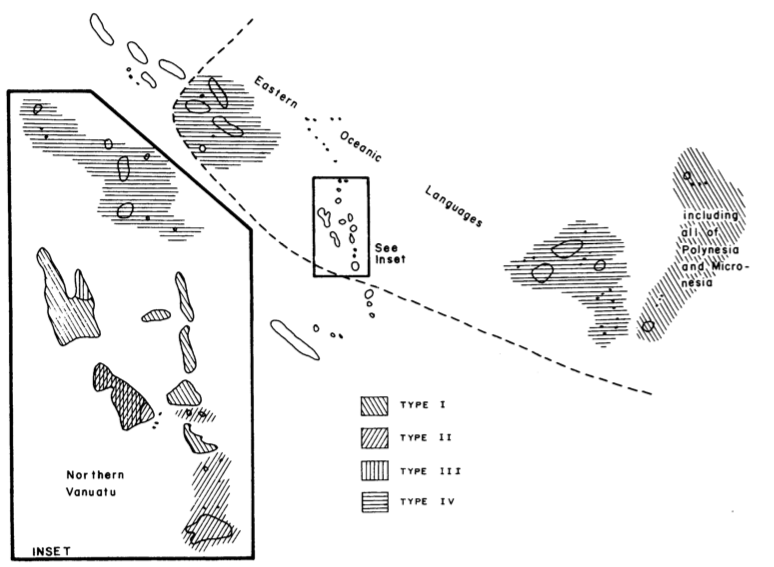
\includegraphics[width=8cm]{illustrations/crowley_1985_map.png}
\caption[Map of four different types of common noun phrase markers in Oceanic from Crowley(1985).]{\textbf{Map of four different types of common noun phrase markers in Oceanic from \citet[162]{crowley1985common}. Type 1: absence of common noun phrase marker or marker is not a reflex of \emph{*na /*a}, type 2: non-productive system involving a reflex of \emph{*na /*a}, type 3: productive marking involving \emph{*na /*a} as a prefix that is regularly separable from the noun and type 4: productive marking involving \emph{*na /*a} generally existing as a free-standing marker.}}
\label{fig:crowley_map}
\end{figure}

In contrast, the corresponding feature in Grambank is `GB022: \emph{Are there prenominal articles?'} (see Fig.~\ref{fig:gb022_map}). Languages that have \emph{te} (like M\={a}ori) or reflexes of \emph{*na/*a} as articles before the noun both count as ``yes'' (1) for GB022 and those that have no prenominal marker as a ``no'' (0). This Grambank feature splits Crowley's type 1 into two categories, and combines all the languages with reflexes of \emph{*na/*a} and \emph{te} (or other markers) into one category. We can now distinguish those that have a pre-nominal article from those that do not, but we cannot tell apart those which have retained the proto-form from those which have not. Since many reconstructions of grammar in historical linguistics rely on particular forms, this is an important difference. This does not matter for features such as word order.

\begin{figure}
\centering
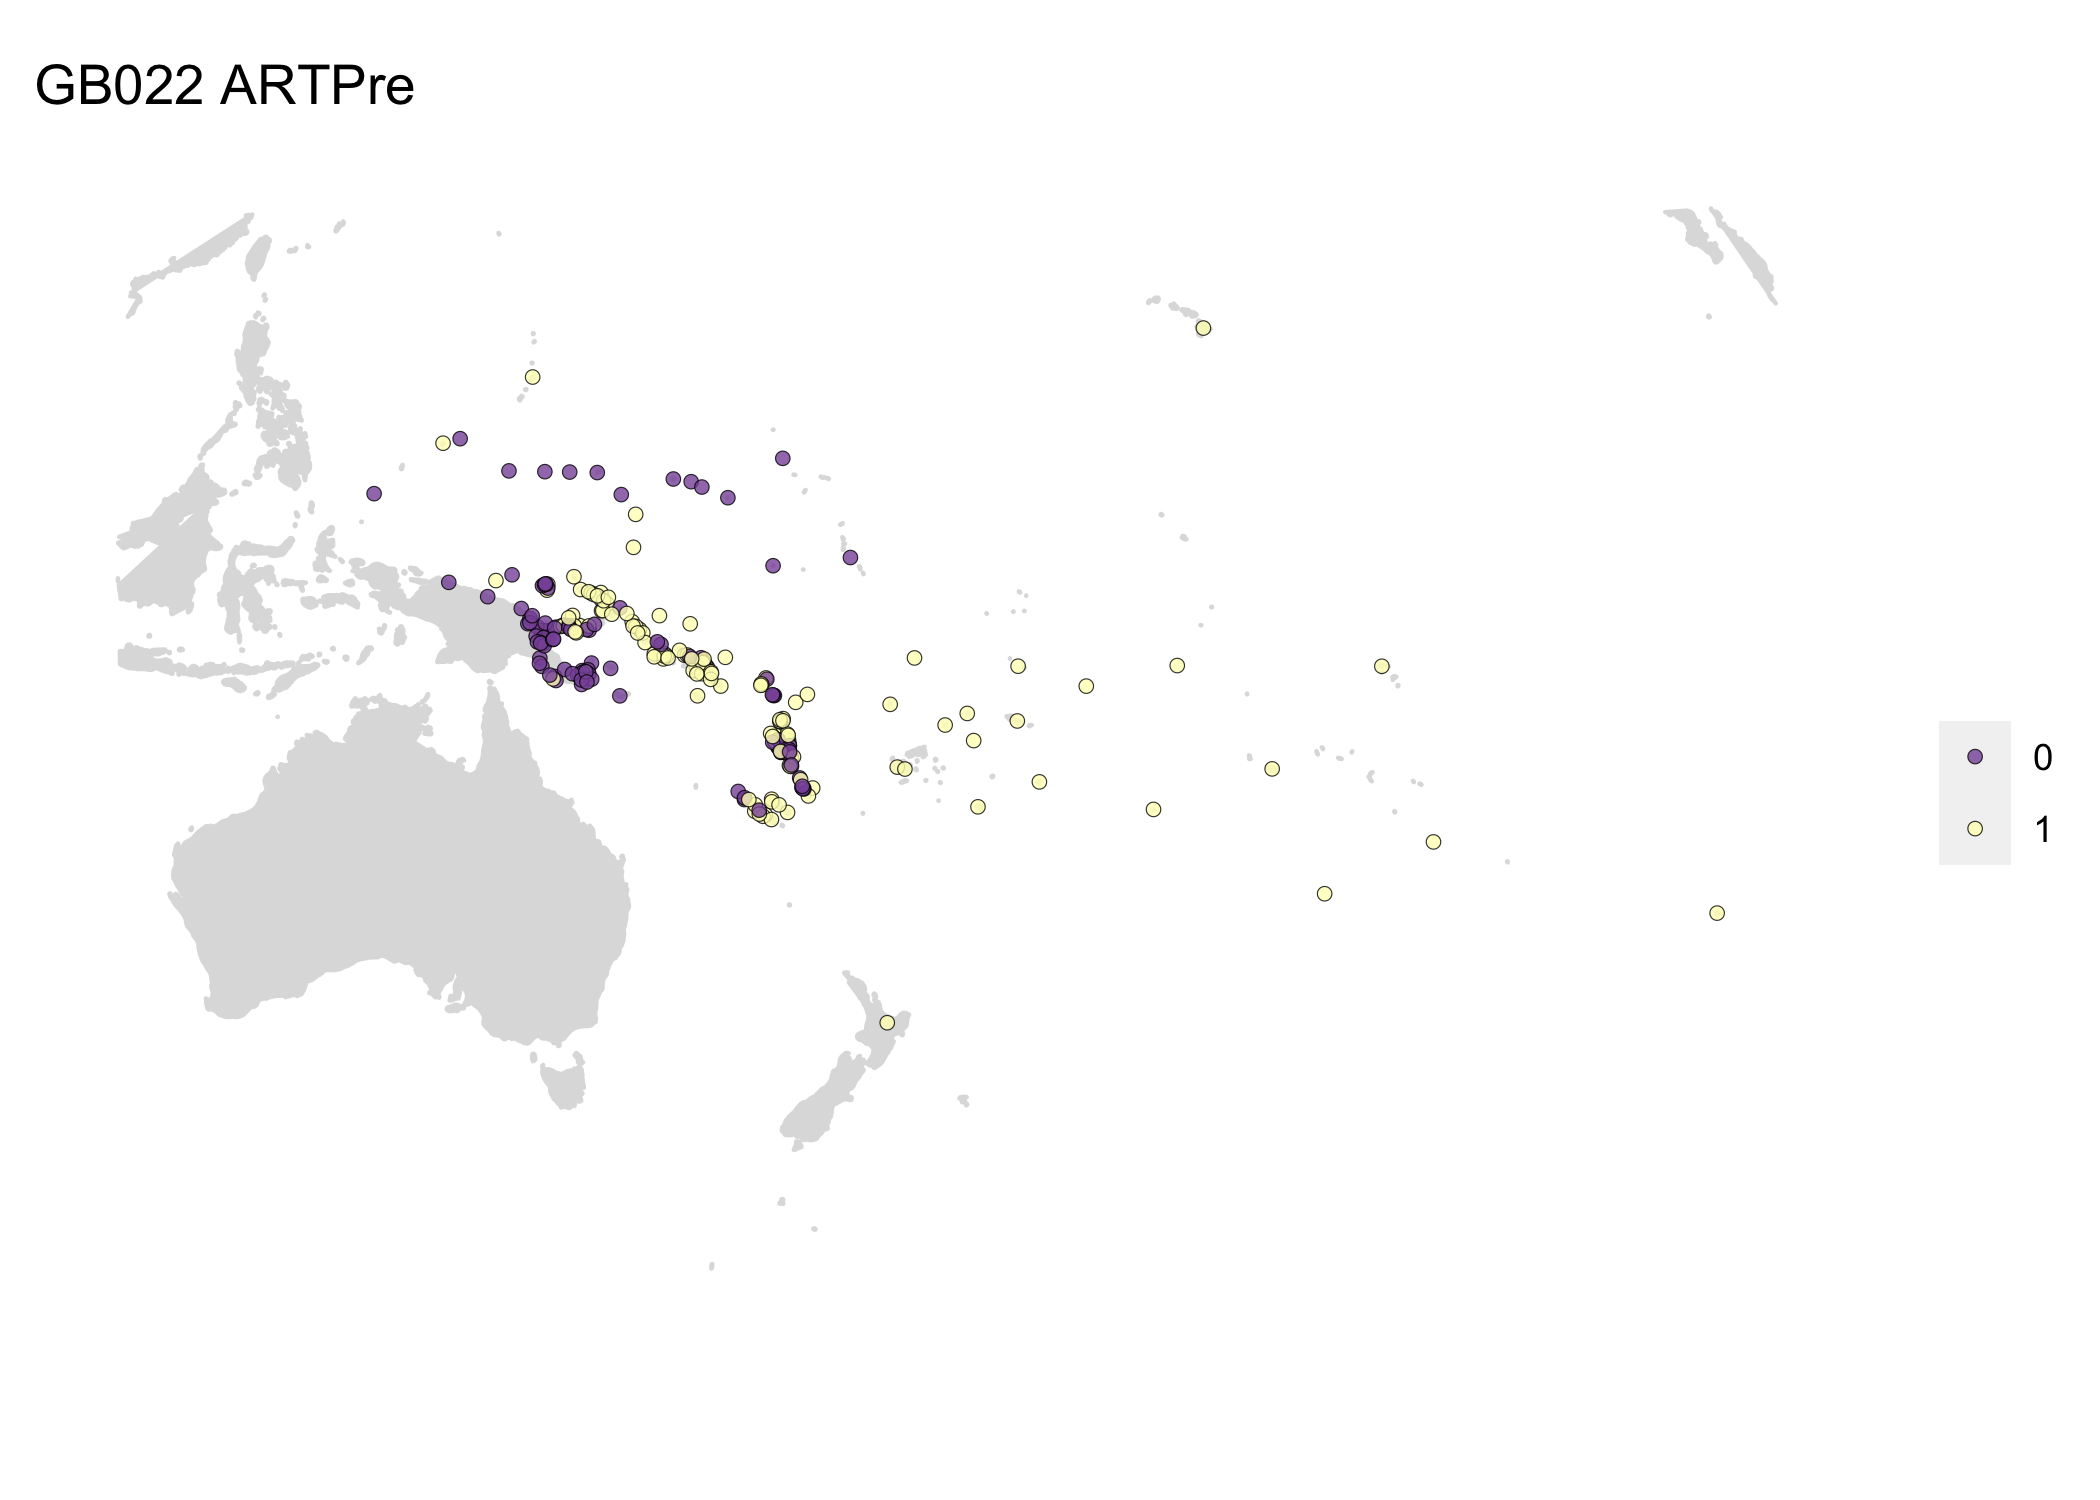
\includegraphics[width=20cm]{illustrations/plots_from_R/coverage_plots/maps/map_GB022.png}
\caption{{Map of Austronesian languages for GB022 \emph{Are there prenominal articles?} Yellow = ``yes", purple = ``no".}}
\label{fig:gb022_map}
\end{figure}

The data in this study is composed of abstract features such as ``is a grammatical distinction made between X and Y?''. This makes it different from most studies of grammatical features in historical linguistics. As was noted earlier, it is possible for two languages to be coded alike but not share ancestry. It is also possible that such abstract features track something beyond the particular forms. \citet[503]{ross2004morphosyntactic} notes that a particular structure of the pronominal system of Mokilese is maintained, despite the formal markers being continuously replaced. He argues that there are discourse related reasons for maintaining this system and that the interaction between this construction and the rest of the grammar is such that the distinction is maintained. When particular markers are lost in this system, new ones appear in their place\footnote{He also notes that Goddard has observed similar patterns in Algonquian languages \citep{goddard1993algonquian}.}. This may be true of more features, and in such cases languages can share a grammatical feature but not have the same particular expression, and this could be due to inheritance. In addition, in many instances --- particularly within families --- abstract features such as 'GB022: \emph{Are there prenominal articles?}' are in fact correlated with specific forms even if the forms are not explicitly being tracked.

%Furthermore, it is possible that due to the interconnectedness of structural features related languages can develop similarily without 
%Related languages may also show similarity due to inheritance, even if the relevant state was not present in the ancestor, as the quote from \citet{chung1977aspects} earlier continues:

%\begin{quotation}
%\noindent\emph{[I]t is also reasonable that changes begun in a Proto-language may have continued even after its separation into daughter languages. In this way, related languages may come to share a feature which existed only in embryonic form, or not at all, in their common ancestor}\footnote{This idea is important to a particular hypothesis about Proto-Polynesian syntax, because according to \citet{chung1978} Proto-Polynesian was accusative and Tongan and S\={a}moan both developed ergativity semi-independently while the Eastern Polynesian languages (which are more closely related to S\={a}moan than to Tongan) did not develop this feature.}.
%\end{quotation}
%\begin{flushright} \citet[539]{chung1977aspects} \end{flushright}
%
%This theory proposes that the conditions for developing a certain feature may have been present in the ancestral language even if the feature itself is absent. It is therefore likely that the daughter languages would develop it even if they were isolated from each other, because they have inherited the prerequisites for developing the feature. This is similar to what is known in the literature on cultural evolution as ``preadaptation'' \citep{scott2010language}. One might say that the seed is sown already in the parent language, and that as a result its daughter languages will likely turn out a certain way.
%
%This ties in with the dependencies of features, insofar as dependencies are representations of features ``moving as a group'' through time. If some of these features are reliable ``early movers'', one could use them to predict certain developments in daughter languages. This theory aligns well with a view of language as a system where everything neatly fits (``La langue est \emph{un système où tout se tient}'' [language is systematic / a system where everything fits], Saussure \citep{koerner1997notes}). This is in contrast to the view by, among others, \citet[328]{bloomfield1933language} who stated that \emph{every word has its own history}. It is likely that systematic effects like these are more probable in structural data than in lexical data.
%
%However, in this analysis we are investigating each feature separately so it is not possible to derive information about features co-evolving. It is also difficult for the algorithm \emph{not} to reconstruct a certain state in the parent language, if the majority of daughter languages possess it. This is one instance where knowledge of plausible paths and profiles of languages from classical linguistics may contribute information that is, so far, not possible to retrieve using computational means.

%In summary, the comparative method of historical linguistics involves Maximum Parsimony coupled with information on plausibility. It is not possible in computational reconstruction to take plausibility into account since it has not been formalised. The kind of data typically used in reconstruction of grammar in historical linguistics concerns specific forms, whereas the data for this paper is structural features.

\section{Material and methods}
\subsection{Computational phylogenetic methods}
\label{sec:asr_methods}

In this study, we will be reconstructing the presence or absence of structural features in proto-languages of the Oceanic subgroup using Maximum Parsimony and Maximum Likelihood. This section gives a brief overview of the methods. Further technical details concerning the precise application can be found in the supplementary material \ref{supp:tech_details}. For an extensive comparison of different methods of ancestral state reconstruction and their advantages, see \citet{joy2016ancestral}.

As discussed earlier in section \ref{sec:ars:metod:hist}, \textbf{Maximum Parsimony} finds the set of ancestral states that result in the fewest number of changes between nodes. Maximum Parsimony is intuitively simple. We saw in the previous section an example of how it can play out in a small tree. While the principle of ``Maximum Parsimony'' is practised in traditional historical linguistics as a part of the Comparative Method, it should be noted that they rarely use the term \emph{per se}, but rather the description of ``fewest number of changes along the tree''.

Maximum Parsimony may be simple and intuitive, but it is not without its critics. Part of the critique is that it does not take into account branch lengths in the tree (the time between splitting events). Furthermore, Maximum Parsimony necessarily assumes that the solution that posits the slowest possible rate of change is also the most probable one. This is not necessarily a valid assumption; some features may evolve at a faster rate than Maximum Parsimony predicts. Both of these disadvantages are addressed in the second method we will be applying: Maximum Likelihood.

%The second method which will be applied in this study is that of \textbf{Maximum Likelihood}. 
Ancestral state reconstruction using \textbf{Maximum Likelihood} posits the most likely ancestral state distributions based on the overall probabilities given all the nodes in the tree and all branches. This approach does not assume that the slowest rate of change is the most probable one. If, for example, the distribution of values at the tips is very scattered, with sibling pairs frequently having different values, Maximum Likelihood will infer that the feature has a high rate of change and use that information when positing ancestral states as well. The Maximum Likelihood algorithm assigns probabilities of state changes and distributions based on branch lengths. A mutation along a shorter branch is given more weight in the likelihood calculations than if it occurred in a longer branch. Furthermore, reconstruction using Maximum Likelihood allows us to use a model of change where we do not assume that the rates for losses (1$\rightarrow$0) are equal to the rate of gains (0$\rightarrow$ 1). In this study, we use an ``All Rates are Different" (ARD) model, which allows for the rate of loss and gain to be different\footnote{
Similarly to the studies by \citet{carling2021reconstructing} and \citet{goldstein_2022}, rates cannot vary within the tree.}. 

It is not possible for the computational implementation of Maximum Parsimony to take into account branch lengths, nor can it assume anything but the slowest rate of change or posit different rates for losses and gains. It is however possible that the Comparative Method in historical linguistics estimates something similar when they take into account the ``plausibility of the changes posited'' and that this is picked up by the reconstruction by Maximum Likelihood. It is possible that scholars of historical linguistics take length of time into account, for example, or assume that a loss is more likely than a gain for a given feature. In this study, we compare Maximum Parsimony and Maximum Likelihood reconstructions to the Comparative Method. If the results from the Comparative Method are more similar to that of Maximum Likelihood, a potential explanation would be that the ``plausibility of changes posited'' is indeed operating along similar lines as Maximum Likelihood by taking branch length into account and assuming varying rates of change.

Finally, we will also compare the predictions of historical linguists with computational predictions based solely on which value is the most common in the daughter languages of a given proto-language --- entirely disregarding the tree structure\footnote{This is similar to the frequency heuristic described in \citet{goldstein_2022}.}. In the toy example in Fig. \ref{fig:clark_tree}, this approach would reconstruct that the root had feature value ``X''. Whether we prefer Maximum Parsimony, Maximal Likelihood or another approach to reconstruction, it should be the case that actually taking the tree structure into account is the sounder methodology. %We expect that both methods has a higher degree of concordance with the findings in historical linguistics compared to only counting which value is most common.

%The third method employed is \textbf{Stochastic Character mapping}. This method was proposed by \citet{huelsenbeck2003stochastic} and is an extension of an approach suggested by \citet{nielsen2002mapping}. 
 
\subsection{Calculation of similarity between predictions from the Comparative Method and computational approaches}
\label{result_calc_section}
We calculate the similarity of the predictions of historical linguists and computational means with two measures: concordance and F1-scores. Concordance is known as \textit{accuracy} in machine learning, but we wish to avoid the connotation that what is being measured is the accuracy of the reconstruction as regards real languages. Rather, concordance measures how closely the computational reconstruction matches historical linguists' reconstruction. It is measured as the number of agreements about grammatical features (i.e. Grambank binary questions) of predicted protolanguages, divided by the total number of grammatical features predicted. 

F1-scores are the harmonic mean of the precision and recall\footnote{Precision is True Positives divided by True Positives + False Positives, recall is True Positives divided by False Negatives + True Positives. F1-score = 2 * ((precision*recall) / (precision + recall)) \citep{van1979information}.} \citep[133]{van1979information}. It is important to note that F1-scores disregard the number of True Negatives entirely, which is relevant in our case since some of the features in proto-languages are predicted to be absent. For both measures, 0 is the worst possible score and 1 the best in terms of similarity to predictions by historical linguists. 

In a similar study of ancestral states of cognate classes, \citet{jager2018using} compared three different methods of ancestral state reconstruction for lexical data (cognate classes): Maximum Parsimony, Maximum Likelihood and Minimal Lateral Networks. They found that reconstructions using Maximum Likelihood performed the most like the predictions by historical linguists. However, \citet{jager2018using} describe the general performance of all the computational reconstruction methods they used as ``poor''.  \citet{jager2018using} evaluated the methods using the F1-score. The highest F1-score was 0.79 (Austronesian language sample, Maximum Likelihood), and the worst was 0.44 (Indo-European, Minimal Lateral Networks).

%In addition to these two scores we will also calculate how much better each method does compared to just counting which is the most common vale of a feature in the daughter languages. As we learned in section \ref{sec:ars:metod:hist}, simply relying on frequency and not taking the tree structure into account can lead us astray. Whether we prefer Maximum Parsimony, Maximal Likelihood or another approach to reconstruction it should be the case that actually taking the tree structure into account is the more sound methodology. We expect that both methods has a higher degree of concordance with the findings in historical linguistics compared to only counting which value is most common.

For each feature, the methods predict a distribution of the two states (presence and absence) for every ancestral node. If the distribution is majority presence (more than 60\% of the ancestral state is ``1'') it is registered in the results as ``Presence''; if less than 40\% presence it is registered as ``Absence''. If the ancestral state is between 40-60\% of either state, the prediction is registered as ``Half/Half''. This was done to highlight the amount of uncertainty the results sometimes contain, while at the same time making it a fair comparison between Maximum Parsimony and Maximum Likelihood. Comparing the raw distributions themselves is not a fair comparison because Maximum Parsimony is always more likely to suggest 0, 0.5 or 1 results whereas Maximum Likelihood rarely produces exactly 0 or 1. 

If the reconstruction of a feature by experts for that ancestral node was ``Presence'' and the algorithm did predict presence with over 60\%, it is counted as a ``True Positive'', and so on\footnote{The terms ``True'' and ``False'' are used here in accordance with terminology in machine learning. In this instance, they are indicating whether the results from the computational method and historical linguists agree. It should not be interpreted as a measure of ``Truth'' necessarily.}. Table~\ref{example_HL_prediction_table_true_positives} illustrates how the results are summarised.

\begin{table}[H]
\centering
\caption{Table illustrating how the results of ancestral node predictions are calculated.}
\label{example_HL_prediction_table_true_positives}
\begin{tabular}{|l|l|l|l|l|l|l|l|}
\hline
\textbf{Finding in historical linguistics} & \textbf{Prediction by Computational Method} & \textbf{Result} \\ \hline
Absence & >60\% Absence & True Negative \\ \hline
Absence & >60\% Presence & False Positive (type 1-error) \\ \hline
Presence & >60\% Presence & True Positive \\ \hline
Presence & >60\% Absence & False Negative (type 2-error) \\ \hline
Absence & 40-60\% Presence/Absence & Half \\ \hline
Presence & 40-60\% Presence/Absence & Half\\ \hline
\end{tabular}
\end{table}

For each method, a plain concordance score (Eq \eqref{eq:accuracy}) and F1-score (Eq. \eqref{eq:F1_score}) is then calculated.

\begin{equation}\label{eq:accuracy}
\frac{\text{True Negative + True Positive}}{\text{True Negative + True Positive + False Negative + False Positive}}
\end{equation}

\begin{equation}\label{eq:F1_score}
\frac{\text{True Positive} }
{\text{True Positive} + \frac{1}{2}\times(\text{False Positive} + \text{False Negative})}
\end{equation}

It is also important to take into account the Half-results. This count represents instances where the method was not able to say with a strong confidence that something was present or absent. The reason it is interesting to separate these out is that while they may indicate a majority result one way, it is not far from suggesting the direct opposite. For example, if one of the methods reconstructs Proto-Oceanic as having a 51\% chance of having ergative marking --- it is not far away from suggesting that this marking is absent. In order to take these type of cases into account the cut-off of 40\%-60\% was set and summarised as "Half" results. We can apply the concordance score and F1-scores to this summary statistic as well, as shown in Eqs. \eqref{eq:accuracy_incl_half} and \eqref{eq:F1_score_incl_half}. See supplementary material \ref{math_supp} for more details\footnote{I am very grateful for mathematical assistance from Stephen Mann.}.

\begin{equation}\label{eq:accuracy_incl_half}
\frac{\text{True Negative + True Positive} + \frac{\text{Half}}{2}}{\text{True Negative + True Positive + False Negative + False Positive + Half}}
\end{equation}

\begin{equation}\label{eq:F1_score_incl_half}
\frac{\text{True Positive} +  \frac{\text{Half}}{2}} 
{\text{True Positive} + \frac{1}{2}\times(\text{False Positive} + \text{False Negative}) + \text{Half}}
\end{equation}


All four scores will be reported, but we will rely mainly on the Concordance score with the inclusion of the Half-results. This is because this approach takes into account the True Negative (which F1-scores ignore) and it takes into account the possible uncertainty of the half-scores.


% mutate(F1_score = 2 * ((Precision*Recall)/(Precision + Recall)), 
  %         F1_score_incl_half = 2 * ((Precision_incl_half *Recall_incl_half)/(Precision_incl_half + %Recall_incl_half)) )%>% 
 


%In order to evaluate the results, we need to calculate a concordance score per method and tree. \citet{jager2018using} use the F1-score (harmonic mean between precision and recall) in their study of how computationally reconstructed lexical proto-forms compare to those reconstructed by historical linguists.  For example, if for a given proto-language there are 60 features reconstructed by experts and the algorithm result is 10 True Positives, 10 False Positives, 10 True Negatives, 10 False Negatives and 20 ``Half/Half'' then the F1-score is 0.5 (recall = 10 / (10+10) = 0.5, precision = 10 / (10+10) = 0.5 and F1-score = 2 *((0.5*0.5) / (0.5 + 0.5) = 0.5)). Note that the F1-score disregards True Negatives and Half /Half-results.

%F1-scores will be reported because they are insightful and have been used in similar studies. However, the F1-formula ignores the amount of True Negatives and Half/Half results. Therefore, in addition we will also calculate a simpler concordance score; how many concordant predictions did the algorithm make given all the predictions it made (aka ``accuracy'')? For example, if for a given proto-language there are 60 features predicted by experts with the same distribution of results as in the example above, then the concordance score would be (10 + 10)/40 = 0.5. We can also include the Half/Half-predictions, awarding 0.5 points for at least not strongly predicting a false value. In that case, this example has a concordance score of 0.5 ((10 + 10 + (20/2)) / 60). These scores all reflect different ways of assessing concordance and will give different perspectives on our results and how our algorithms are performing. %Features where there were more than half of the data-points missing in the tree were not to be included. hankfully there were no occurrences of this.

%\begin{equation} \label{accuracy_incl_half}
%\frac{\text{agree} + \frac{\text{half}}{2}}{\text{all reconstructions}}
%\end{equation}

\subsection{Data}

\subsubsection{The Grambank-dataset}
\label{asr:sec:GBcoverage}

The data for the study is taken from the Grambank-project \citep{grambankwebsite}. The Grambank dataset consists of 195 structural features which have been coded by a large group of research assistants for over 2,000 languages. This dataset includes 280 Oceanic languages. 

%The Grambank project is part of the Glottobank consortium, which is a collaboration between the Max Planck Institute for the Science of Human History in Jena (MPI-SHH), the Australian National University, the Australian Research Council's Centre of Excellence for the Dynamics of Language and the University of Auckland. The project is led by a team of senior linguists (Russell Gray, Simon Greenhill and Quentin Atkinson) and employs student assistants as coders in Kiel, London, Canberra, Uppsala and a few other locations. Coders who have been contributed significantly to the database are included as co-authors of the upcoming release paper \citep{grambank_release}, alongside other contributors. I have personally participated in this project as a coder and as a coordinator.

%The aim of Grambank is to provide a consistently coded set of structural features of the world's languages for research questions relating to history, complexity and more. The dataset will be published openly. 
 
%The Grambank dataset builds on previous typological work by \citet{dunnetal2005, dunn2008, reesinketal2009, dunnreesink2012} and \citet{ntswebsite}. The project has a global focus and the aim is to include all languages in the world that are described for their core grammatical structure. 

% In the work by Dunn, Reesink and colleagues, they were particularly focussed on languages of Oceania and Australia and the prehistory of migrations and contact there. The Nijmegen Typological Survey-project \citep{nts2014, ntswebsite} on the other hand was focussed on African languages.

The questionnaire's 195 questions cover what are often called the ``core domains'' of traditional grammatical description: word order, possession, negation, tense, aspect, mood, deixis, interrogation, comparatives and more. Features are included in the questionnaire if it is likely that it is possible to answer them for the majority of the world's languages which are at least described in a grammar sketch (approx 4,000 languages). This means that rarer features are not included. The full questionnaire is found in appendix \ref{Grambank_features}. 

The Grambank dataset is coded by student and research assistants under the supervision of expert linguists. For more details on the coding workflow of Grambank, see \citet{slingerland2020coding}. For further details on the dataset, see Supplementary Material ~\ref{supp:dataset_details}.

%It is crucial in a cross-linguistic survey of this kind that the features are applied consistently across all languages of the sample. Within the Grambank-project, we strive towards a high level of consistency between coders. There are many coders employed and we have established work-flows to ensure that the features are applied consistently across languages. New coders are trained in the workflow and linguistic definitions through collaborative coding. Each feature in the questionnaire is accompanied by a helpful and pragmatic definition in a wiki-page. Each feature is also associated with a ``patron'', an expert linguist assigned to a set of features who has the final word should any further clarification be needed or disagreements arise. There are seven patrons in the project: Alena Witzlack-Makarevich, Harald Hammarström, Hannah Haynie, Jeremy Collins, Jay Latarche, Jakob Lesage and myself. All coders in the project are able to converse with each other and patrons through GitHub, an online platform for project coordination and code collaboration. When we are unable to make a coding decision with sufficient confidence, the data-point is marked as ``?''.


\subsubsection{Data coverage} 
This study is focussed on the Oceanic subgroup of the Austronesian language family. The Oceanic subgroup covers almost all languages in Remote Oceania (with the exceptions of Chamorro and Palauan) and large parts of Near Oceania. Fig.~\ref{Oceanic_map} from \citet[2]{protooceanicvol5} shows the extent of the major subgroups of the Austronesian language family, with Oceanic covering the largest surface area. Following the language classification of Glottolog 4.0 \citep{glottolog40}, there are 522 languages in total in the Oceanic subgroup.

\begin{figure}[h]
\centering
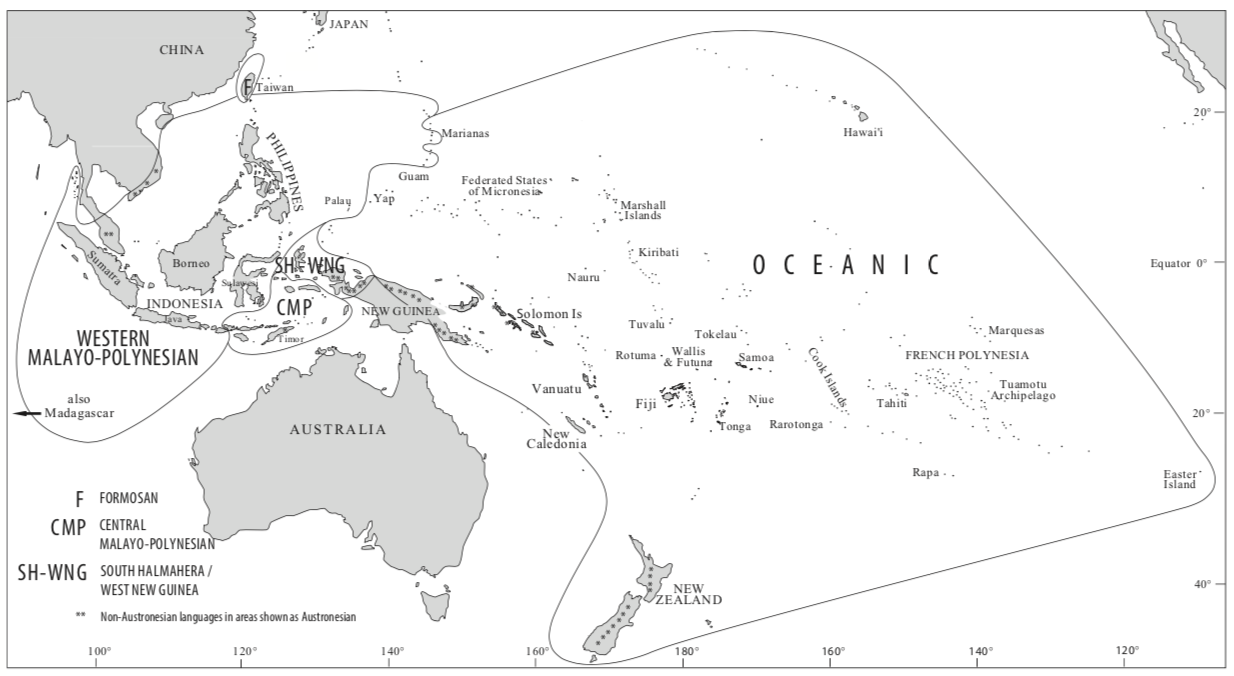
\includegraphics[width=\textwidth]{illustrations/ross_pawley_osmond_protooceanic_vol5.png}
\caption{{Map of the Austronesian language family and major subgroups, from \citet[2]{protooceanicvol5}.}}
\label{Oceanic_map}
\end{figure} 

Not all languages of the Oceanic subgroup have a grammatical description, but out of those that have it nearly all are included in Grambank. Table~\ref{GB_coverage_table_island_group} shows the coverage of Oceanic languages in the entire dataset. According to Glottolog, there are 289 Oceanic languages that have a grammar or grammar sketch which means that they can be included in Grambank at all. It is not always possible to fill in all the features for every language. Twenty of the Oceanic languages that are included to date are less than 50\% completed for Grambank questions. This can be due to lack of access to descriptive work, or that the content of the descriptive work does not cover the necessary domains in enough detail for the coders to answer enough questions. The map in Fig.~\ref{GB_austro_coverage} shows the same coverage information, with languages coded for their data coverage status.

\newpage
% latex table generated in R 4.2.0 by xtable 1.8-4 package
% Wed Jun 22 18:04:34 2022
\begin{table}[ht]
\centering
\begin{tabular}{p{5cm}p{2.7cm}p{2.7cm}p{2.7cm}p{2.7cm}}
  \hline
Island group & grammar doesn't exist & grammar exists (not in GB, yet) & Less than half of features covered in GB & More than half of features covered in GB \\ 
  \hline
Bismarck & 5 & 1 & 7 & 42 \\ 
  Central Pacific & 11 & 0 & 1 & 33 \\ 
  Central Vanuatu & 42 & 0 & 1 & 48 \\ 
  Interior New Guinea & 11 & 0 & 0 & 4 \\ 
  Micronesia & 6 & 0 & 1 & 16 \\ 
  N Coast New Guinea & 77 & 2 & 3 & 19 \\ 
  New Caledonia & 18 & 1 & 0 & 14 \\ 
  Northern Vanuatu & 9 & 0 & 0 & 5 \\ 
  S New Guinea & 36 & 3 & 1 & 26 \\ 
  Solomons and Bougainville & 25 & 1 & 4 & 30 \\ 
  Southern Vanuatu & 1 & 0 & 0 & 8 \\ 
  Temotu & 3 & 0 & 2 & 5 \\ 
  Total & 244 & 8 & 20 & 250 \\ 
   \hline
\end{tabular}
\caption{Table showing coverage of Oceanic languages in Grambank per island group with matches to the Gray et al 2009-tree} 
\label{GB_coverage_table_island_group_gray}
\end{table}

\newpage

\begin{sidewaysfigure}[H]
\centering
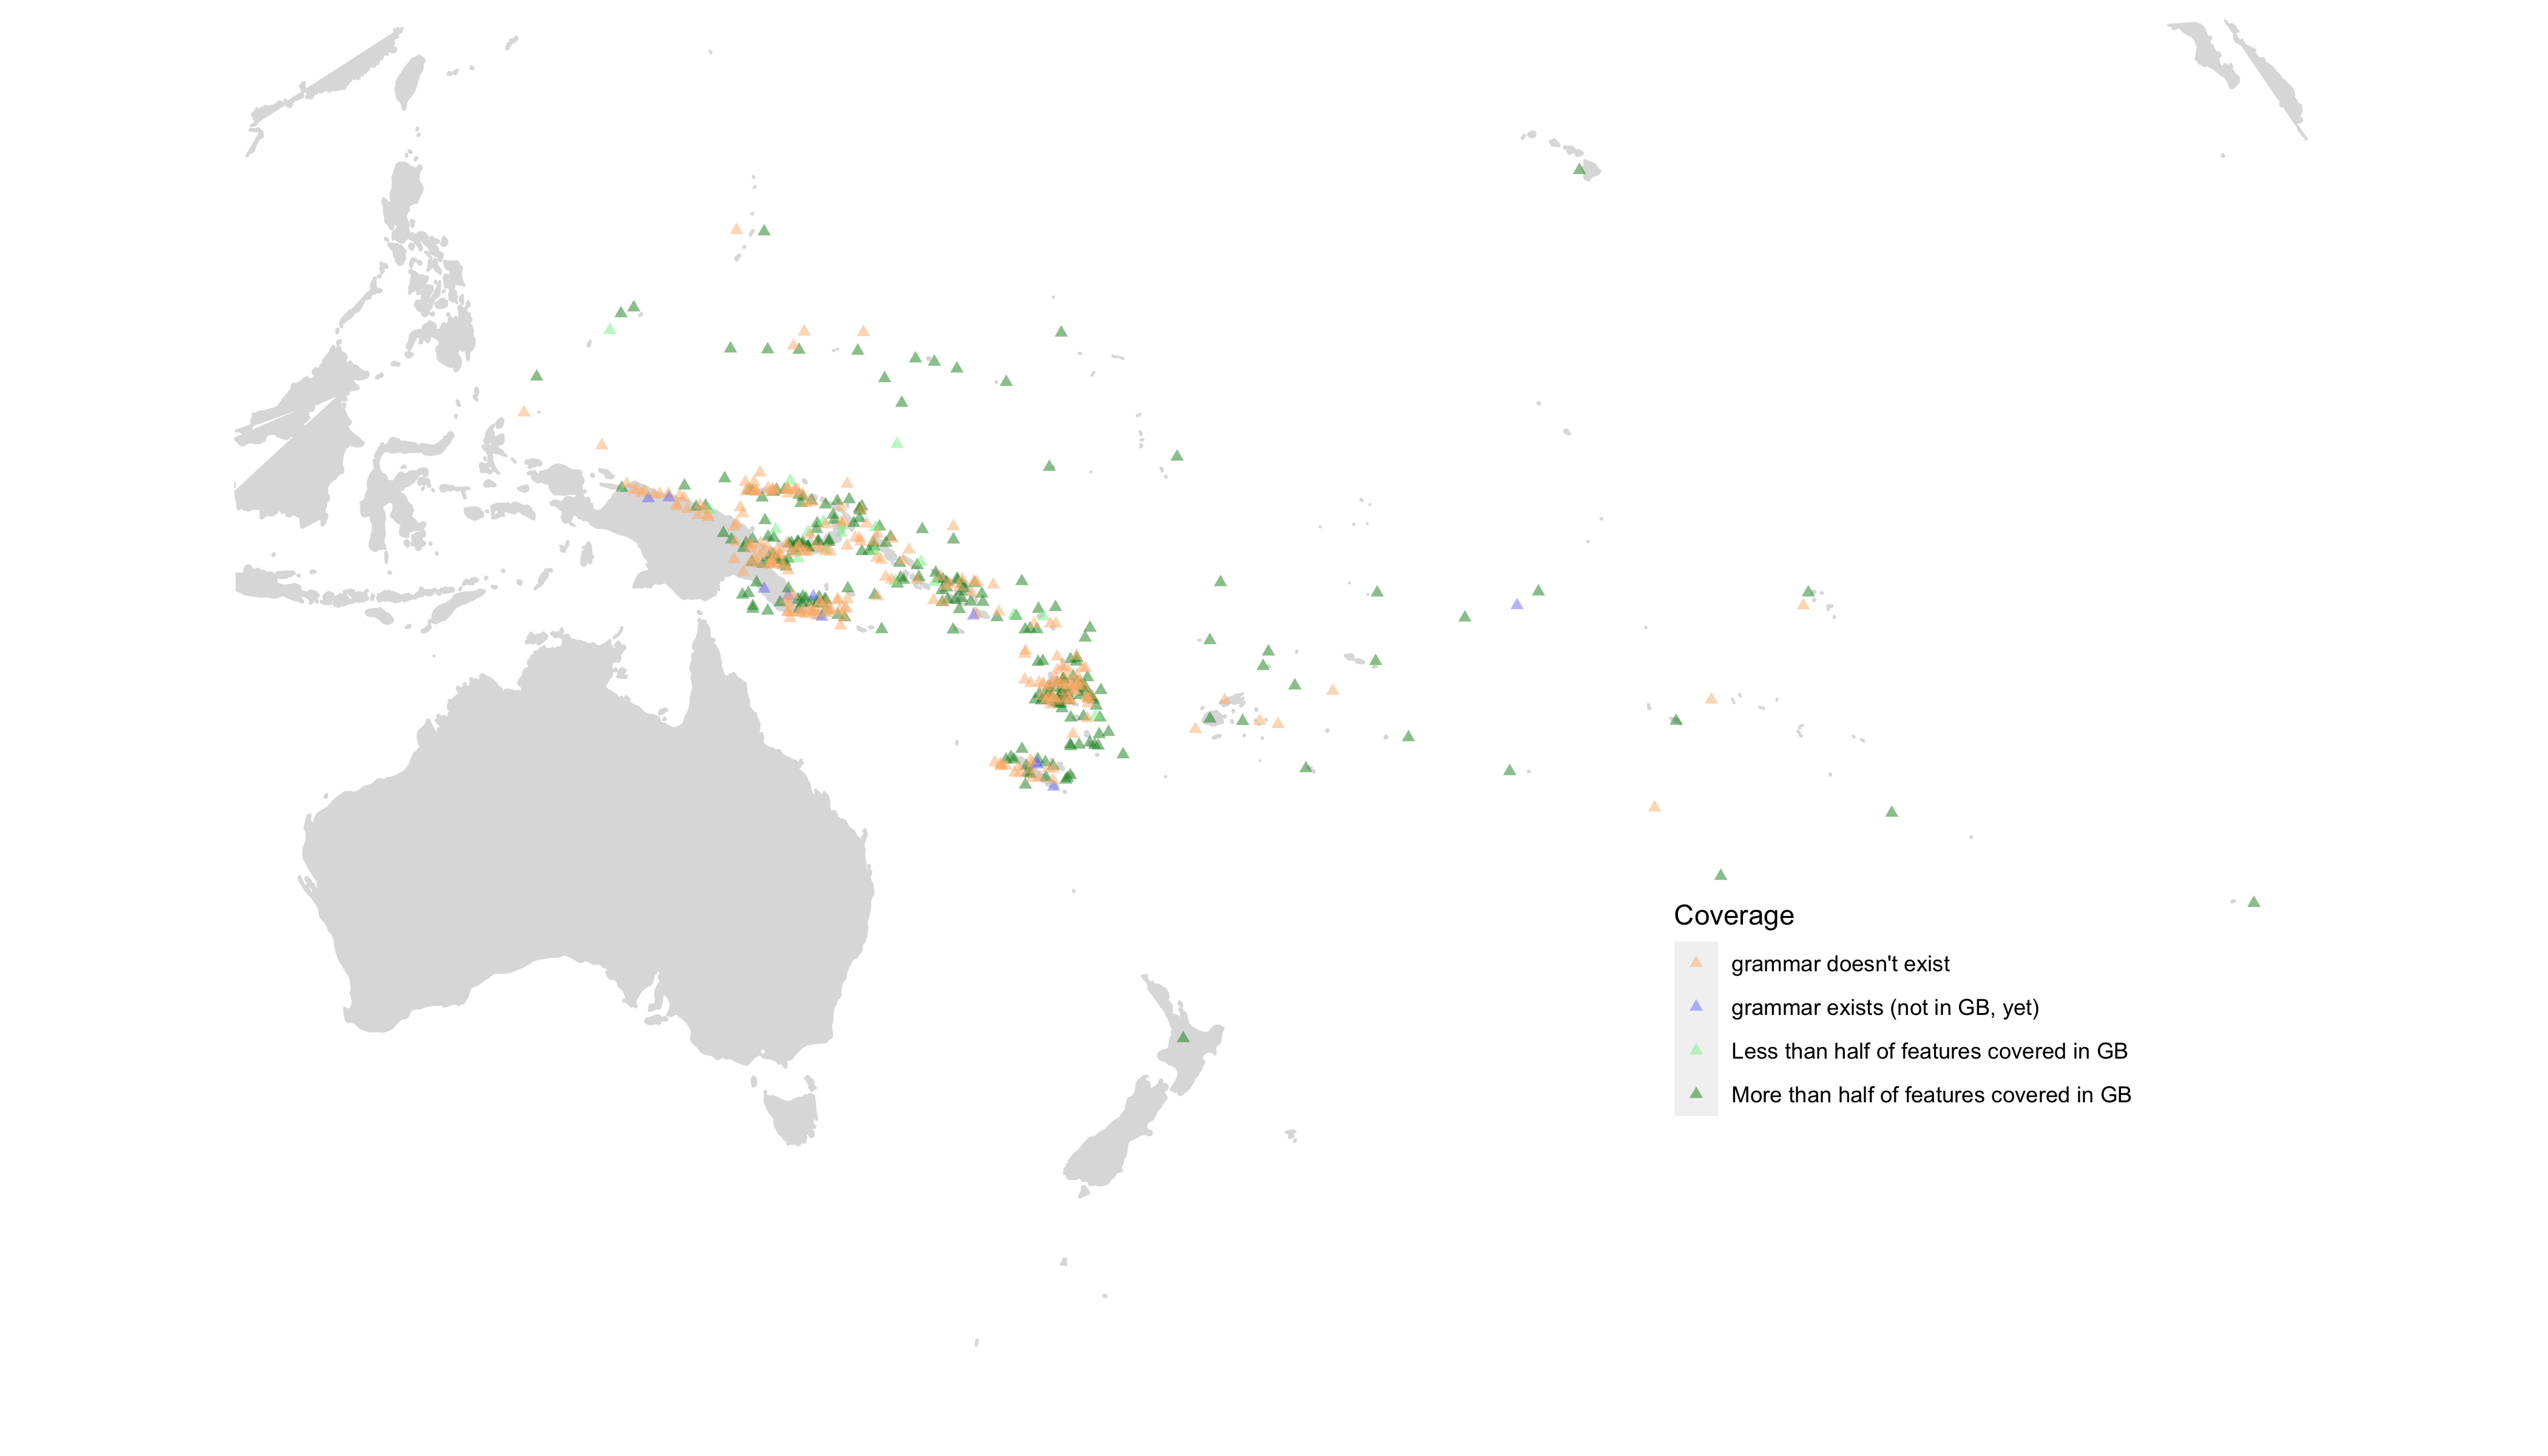
\includegraphics[width=\textwidth]{illustrations/plots_from_R/coverage_plots/maps/coverage_map_oceanic.png}
\caption{{Map of Oceania, with Oceanic languages coloured for their coverage in Grambank.}}
\label{GB_austro_coverage}
\end{sidewaysfigure} %#update

The coverage of Grambank data for the Oceanic subgroup is in general better in the east than in the west. However, since we control for genealogical relatedness through the distance control approach, this is less of a problem for our methodology than if we were using traditional probability sampling (c.f. \citet{ross2004morphosyntactic}).

\subsubsection{The trees}
The tree phylogenies used in this study are: a) the Maximum Clade Credibility Tree (MCCT) from \citet{grayetal_2009}; b) a random sample of 100 posterior trees from the same source; c) the tree from Glottolog 4.0\footnote{The tree of Glottolog 4.0 \citep{glottolog40} is based on work by \citet{blust_2009, blust_2014} and \citet{blust_chen_2017}.}. 

Figure ~\ref{tree_coverage_oceanic_gray} and Figure ~\ref{tree_coverage_oceanic_glottolog} show the Grambank coverage of languages over the phylogenies from the Gray et al 2009-MCCT-tree and the Glottolog-tree respectively. 

\begin{figure}[H]
\centering
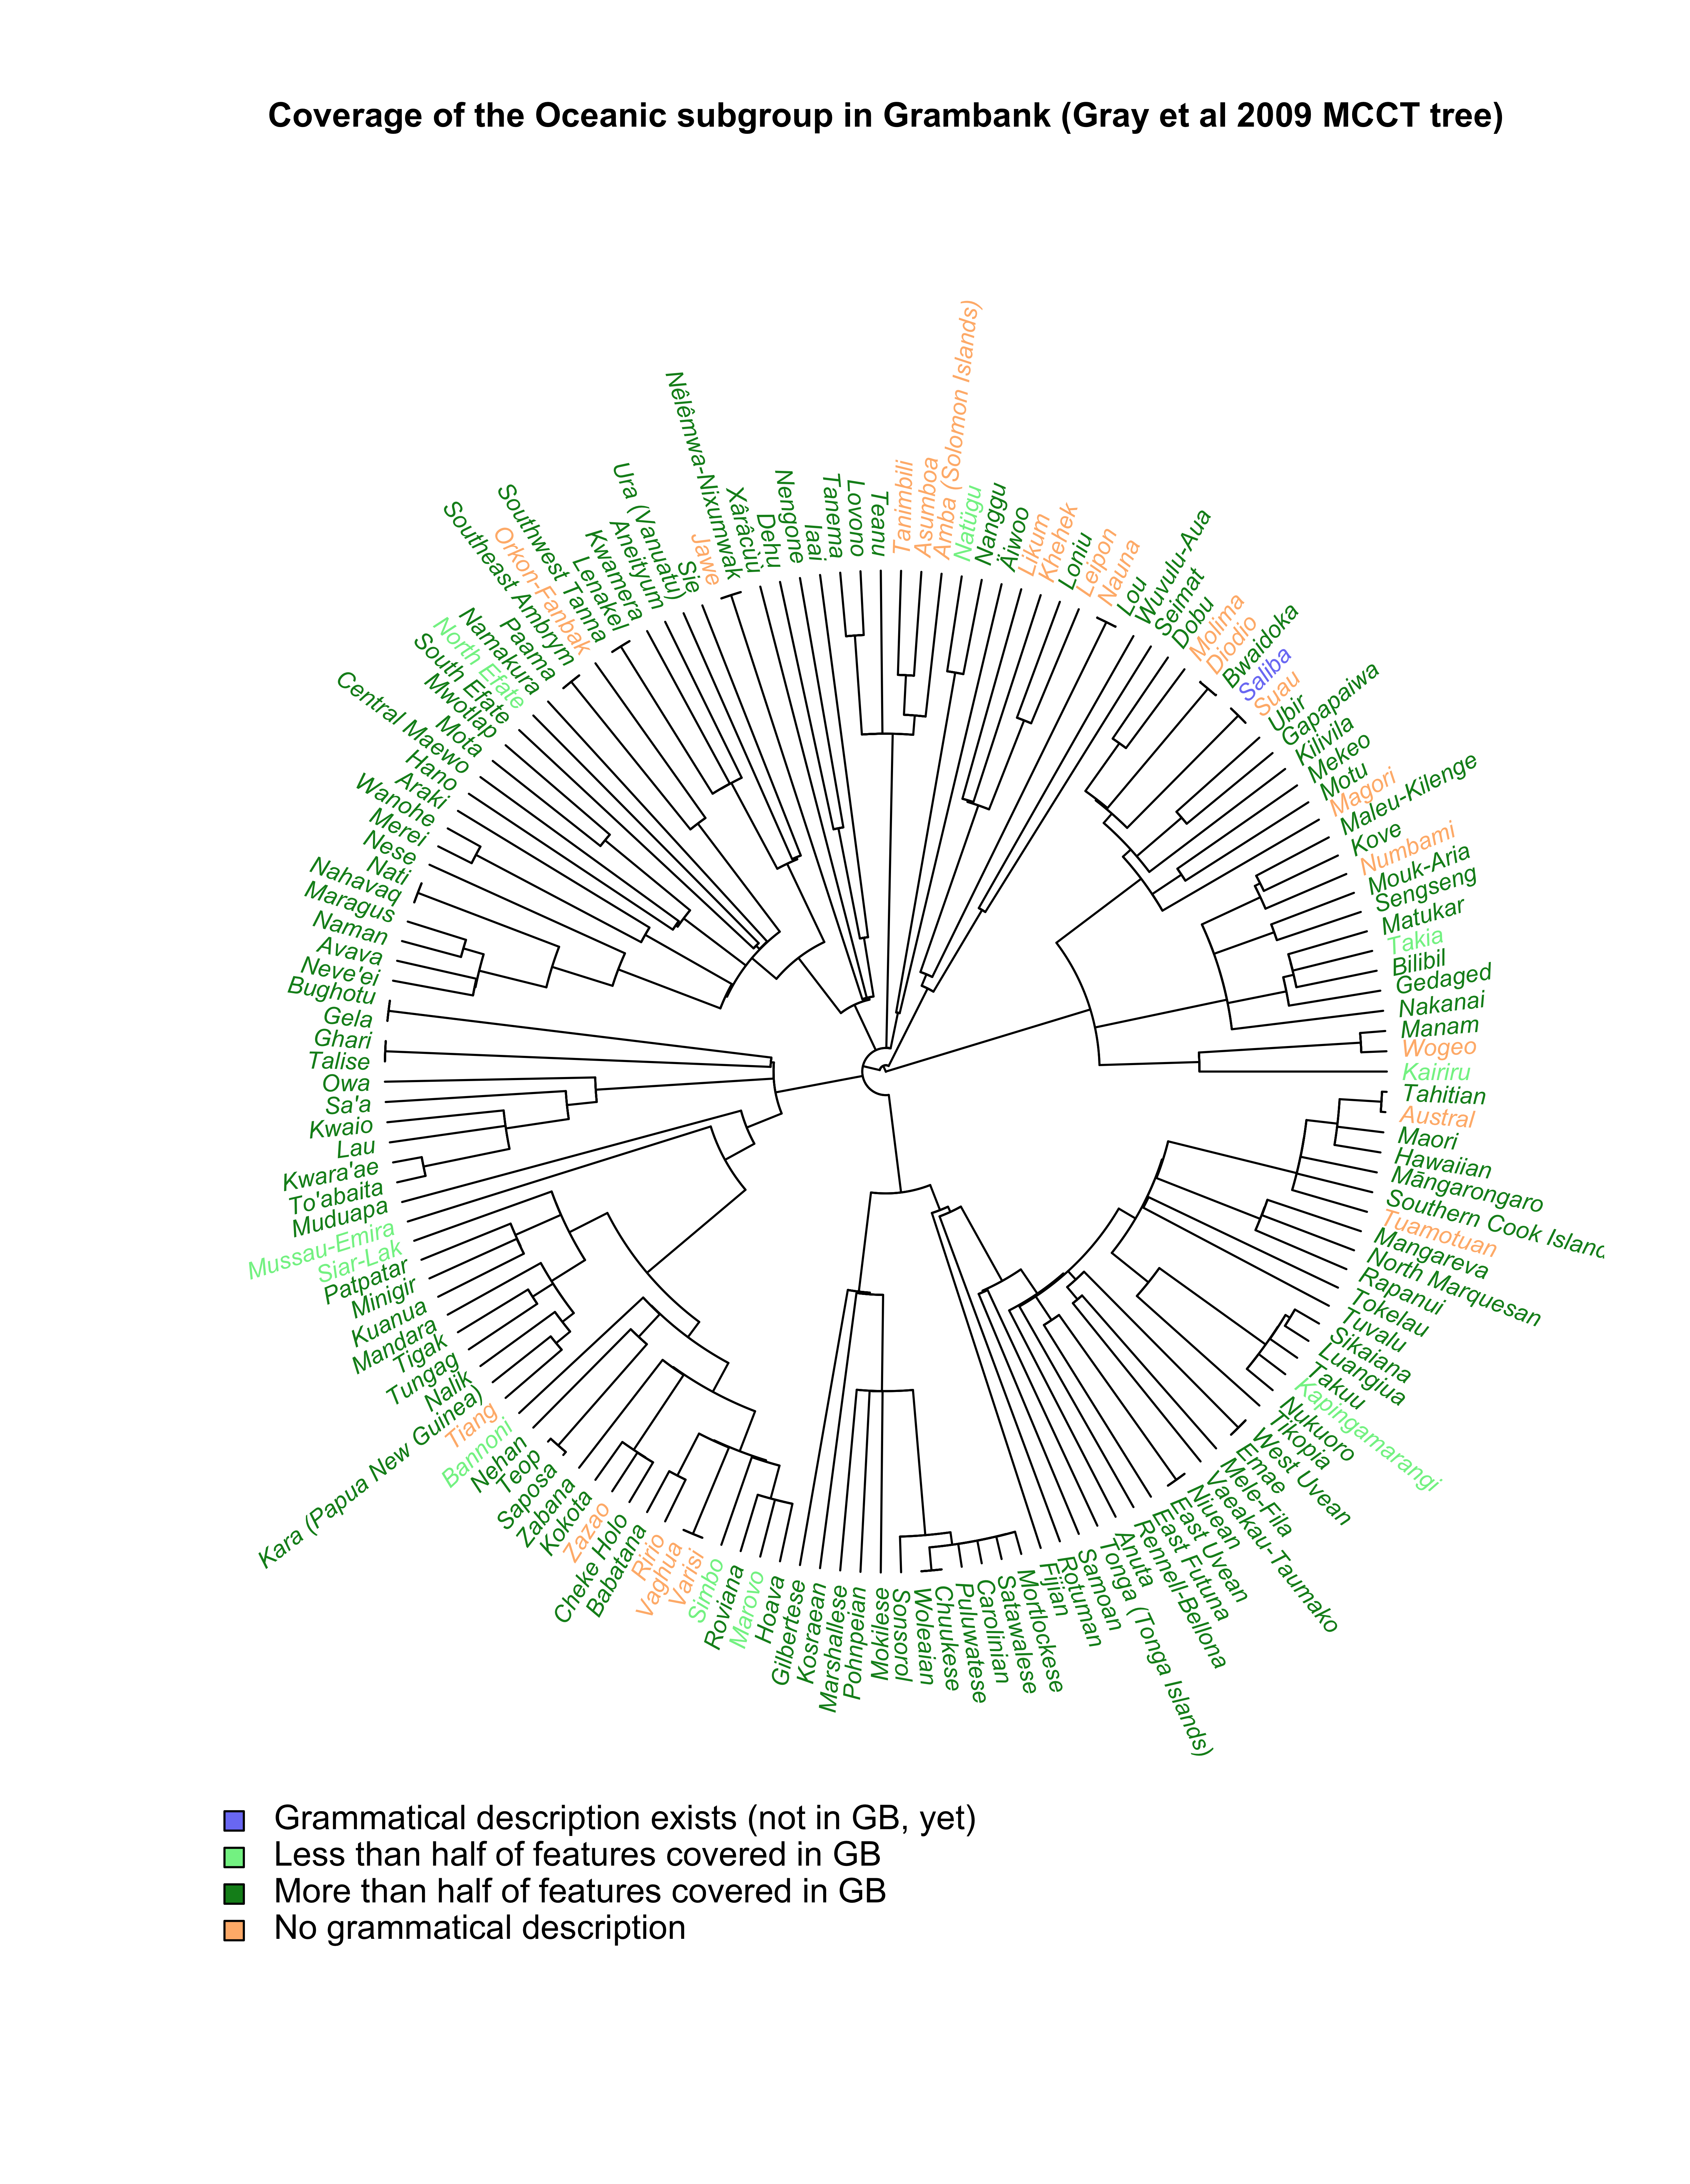
\includegraphics[width=\textwidth]{illustrations/plots_from_R/coverage_plots/tree/Oceanic_tree_desc_status_gray_et_al_tree_mcct.png}
\caption{{Maximum Clade Credibility Tree of Oceanic from \citet{grayetal_2009}, with languages coloured for coverage in Grambank.}}
\label{tree_coverage_oceanic_gray}
\end{figure}

\begin{figure}[H]
\centering
\includegraphics[width=\textwidth]{illustrations/plots_from_R/coverage_plots/tree/Oceanic_tree_desc_status_glottolog_tree.png}
\caption{\textbf{Tree of Oceanic from Glottolog, with languages coloured for coverage in Grambank.}}
\label{tree_coverage_oceanic_glottolog}
\end{figure}

One of the major differences between the trees is that the Glottolog-tree does not contain \emph{any} information about branch lengths. All the branches in the Glottolog-tree are of the same length (1), whereas the branches in the Gray et al 2009-trees (the MCCT and the posteriors) have meaningful branch lengths based on rates of change in the underlying data (basic vocabulary) and calibration points (archaeological dates). This can be seen in the visualisations in Figures ~\ref{tree_coverage_oceanic_gray} and \ref{tree_coverage_oceanic_glottolog} where the first has varying lengths of branches but the latter all have a uniform length (1). This has the consequence that some tips in the Glottolog-tree are much further from the root than others. This is a big disadvantage with this type of tree, since it suggests that different amounts of time has passed between the root and the languages at the tips. Further technical details of the trees can be found in Supplementary Material ~\ref{supp:tree_details}.

The Glottolog-tree contains all the languages in the Oceanic subgroup. Therefore the coverage per island group that is summarised in table ~\ref{GB_coverage_table_island_group} in the previous section applies to the Glottolog-tree as well. However, the \cite{grayetal_2009}-trees do not contain all Oceanic languages, but rather 155. Out of these 132 also occur in the Grambank dataset. %A breakdown of coverage for the\cite{grayetal_2009}-trees per island group is found in table ~\ref{GB_coverage_table_island_group_gray}.

Finally, we are also using a sample of the posterior trees from \cite{grayetal_2009}. Their study yielded 4,200 posterior trees. Tree topologies that are more probable occur more often, but less probable trees also appear in the posterior. By using a set of possible trees instead of just one we can include other possible histories into our analysis, which could for example estimate contact events as well as inheritance. Figure ~\ref{densitree_plot} shows a visualisation of the 100 trees which are used in this study.

\begin{figure}[H]
\centering
\includegraphics[width=12cm]{illustrations/plots_from_R/coverage_plots/tree/gray_et_al_2009_100_sample_densitree.png}
\caption{\textbf{DensiTree \citep{bouckaert2014densitree} visualisation of the 100 random sampled trees from the Gray et al 2009-posterior.} Made with the function densiTree() from the R-pacakge Phangorn \citep{phangorn}.}
\label{densitree_plot}
\end{figure}

\subsubsection{Data from historical linguistics on Oceanic proto-language grammar}
\label{sec:POC_lit_review}

%The Oceanic subgroup is well-studied in historical linguistics, in particular its lexicon (see the book series on the Proto-Oceanic lexicon \citep{protooceanicvol1, protooceanicvol2, protooceanicvol3, protooceanicvol4, protooceanicvol5}, among other publications). There has also been considerable work done on reconstructing the grammar of proto-languages, in particular Proto-Polynesian. See table \ref{HL_prediction_table_summary} in section \ref{sec:POC_lit_review} for a summary of all the sources consulted from classical historical linguistics.

The proto-languages of the Oceanic subbranch of the Austronesian language family are generally well researched in terms of their lexicon and phonology (see the book series on the Proto-Oceanic lexicon \citep{protooceanicvol1, protooceanicvol2, protooceanicvol3, protooceanicvol4, protooceanicvol5}, among other publications). There is also substantial work done on the grammar of Proto-Oceanic using the comparative method. I have summarised several major works in the field and distilled their research into testable hypotheses given the Grambank data and our methods. This section gives an overview of the works included and examples of how they have been incorporated into the study. Table~\ref{HL_prediction_table_summary} lists the publications used for the reconstruction of proto-Oceanic by historical linguists. 

For each of these publications, findings have been extracted that support a certain state of a Grambank feature at a certain node. For example, \citet[4]{marck2000_encyclo} writes that a causative prefix has been reconstructed for Proto-Polynesian (\emph{*faka-}). In the Grambank questionnaire we have the feature GB155 `\emph{Are causatives formed by affixes or clitics on verbs?}'. For the ancestral node that connects all the Polynesian languages, we should expect that for GB155 the state is either wholly or overwhelmingly ``1'' (yes/presence). For simplicity, I have only considered four ancestral languages: Proto-Oceanic, Proto-Central Pacific, Proto-Polynesian and Proto-Eastern Polynesian. The choice to focus on these four in particular was based on the fact that they are the most well-researched proto-languages in the literature. 

%For example,  (an ancestral language of Rotuman and Fijian separately from  Polynesian, Samoan and Northern Outliers excluding Eastern Polynesian). 

The literature suggests that Proto-Oceanic was a language with a pre-nominal definite/specific article \citep[136]{crowley1985common}, a distinction between inclusive and exclusive first person pronouns (\citet[112]{pawley1973some}, \citet[184]{crowley1985common}, \citet[500]{ross2004morphosyntactic}, \citet[67, 75]{lynchrosscrowley_proto_grammar_oceanic}), no gender distinctions in pronouns \citep[498]{ross2004morphosyntactic}, a dual number category in pronouns (\citet[498]{ross2004morphosyntactic}, \citet[69]{lynchrosscrowley_proto_grammar_oceanic} and \citet[173]{pawley1973some}), a distinction between alienable and inalienable possession\footnote{A distinction can be made between three different kinds of possessive classification: alienable/inalienable, direct/indirect and dominant/inactive. For the purposes of Grambank and this study, these are treated as similar enough to be included into the same category.} \citep[69]{lynchrosscrowley_proto_grammar_oceanic}, prepositions (\citet[167]{pawley1973some}, \citet[498]{ross2004morphosyntactic}), subject proclitics and object enclitics on the verb (\citet[498-499]{ross2004morphosyntactic}, \citet[83]{lynchrosscrowley_proto_grammar_oceanic}), possessive suffixes on the possessed noun (\citet[495]{ross2004morphosyntactic}, \citet[155]{pawley1973some}) and a transitivising suffix on verbs (\citet[352]{pawley1970change}, \citet[171]{pawley1973some}, \citet[80, 92]{lynchrosscrowley_proto_grammar_oceanic}). The reconstructions regarding ergativity will be presented separately.

Most of the time, the scholars of Proto-Oceanic are in agreement in their predictions. For example, \citet[142]{pawley1973some}, \citet[292]{ross2007two}, \citet[xiii, 125]{clark1976aspects} and \citet[89]{lynchrosscrowley_proto_grammar_oceanic} all propose that the proto-language of the Polynesian subgroup had a construction marking prohibitive that was different from declarative negatives. However, in some instances there are disagreements. As discussed earlier, one such case is the alignment system of Proto-Polynesian. \citet{clark1976aspects} claims that the system was ergative while \citet{hale_1968}, \citet{hohepa_1967,hohepa_1969} and \citet{chung1978} argue that Proto-Polynesian was accusative and several of the daughter languages developed ergativity later. \citet{kikusawa2002proto} and \citet{ball2007ergativity} also disagree on the alignment of Proto-Central Pacific. Because of this disagreement, the results for the computational ancestral reconstruction for Grambank features regarding alignment of these two proto-languages are presented separately.

In the Grambank project, research assistants read published grammatical descriptions and extract information such that it fits with the definitions of our typological questionnaire (see Supplementary Material \ref{Grambank_features}). This survey of the literature on Proto-Oceanic grammar is essentially the same task. Just as with the literature on reconstructed languages, scholars sometimes disagree on the nature of contemporary languages and how they should best be analysed. It is up to the coder to make calls on which analysis to employ, what can be inferred from the literature and what should be left as unknown. It is possible to squeeze even more findings out of these publications; I have tended to be conservative in my interpretations. Out of the 201 (binarised) features in our questionnaire, 33\% (67) were answerable for Proto-Oceanic given this material. The average completion per language in the whole of the Grambank dataset is 75\%. 

\newpage
\section{Results}

\subsection{Concordance between traditional historical linguistics and computational methods}

We are examining results from three approaches in total: a) Maximum Parsimony, b) Maximum Likelihood and c) Most Common value in daughter languages. For (a) and (b) we are also using three different trees: i) Glottolog, ii) \citet{grayetal_2009} MCC-tree and ii) the mean values of reconstruction of a random selection of 100 (out of 4,200) trees in the Bayesian posterior of \citet{grayetal_2009}. That gives 2 * 3 + 1 results, i.e. 7.

%The match between languages in Grambank and the Gray et al-tree is 112, meaning that results with less than 56 tips are ignored.  %#update

All results have been calculated in \texttt{R} \citep{R} using the packages \texttt{castor} (Parsimony, \citet{louca2017efficient}), \texttt{phangorn} (Parsimony, \citet{phangorn}) and \texttt{corHMM} (Maximum Likelihood, \citet{corHMM}). The packages \texttt{ape} \citep{paradis2004ape}, \texttt{adephylo} \citep{jombart2017package}, phytools \citep{revell2012phytools} reshape2 \citep{wickham2020reshape2} \and tidyverse \citep{tidyverse13} were also used for data wrangling, analysis, summarising and visualising.

%The full table of all predictions (excluding those relating to conflicts) and all results per feature, tree and method can be found in table~\ref{asr_table_appendic} in appendix \ref{ASR_comparison_table}. 

Table \ref{True_post_results_table} shows the number of False, Positive and Half-results for each method and tree\footnote{There was one feature for the ML method and the Gray et al 2009-trees where the computation could not be carried out because all the languages had the same value. In such cases, the function used (corHMM from \citet{corHMM}) gives an error because it cannot compute the rates matrix.}. One of the most striking features in Table \ref{True_post_results_table} is the large amounts of Half-results in the Most common Method --- the method where we simply count directly what is most common in all daughters. This means that there were many instances where this approach, which we know to be unsound, would not confidently be able to predict a presence or absence.
 
% latex table generated in R 4.3.2 by xtable 1.8-4 package
% Thu Nov 30 15:19:36 2023
\begin{table}[ht]
\centering
\begin{tabular}{p{4cm}llllll}
  \toprule
$$\textbf{\parbox{2cm}{\raggedright Method}}$$ & $$\textbf{\cellcolor{spec_color_red!50}{\parbox{1.8cm}{\raggedright False Negative}}}$$ & $$\textbf{\cellcolor{spec_color_red!50}{\parbox{1.8cm}{\raggedright False Positive}}}$$ & $$\textbf{\cellcolor{spec_color_yellow!50}{\parbox{1.8cm}{\raggedright Half}}}$$ & $$\textbf{\cellcolor{spec_color_lightgreen!50}{\parbox{1.8cm}{\raggedright True Negative}}}$$ & $$\textbf{\cellcolor{spec_color_lightgreen!50}{\parbox{1.8cm}{\raggedright True Positive}}}$$ & $$\textbf{Total}$$ \\ 
  \midrule
ML Glottolog & 10 & 3 & 4 & 46 & 52 & 115 \\ 
  ML Gray et al (2009) - MCCT  & 9 & 2 & 9 & 43 & 51 & 114 \\ 
  ML Gray et al (2009) - posteriors  & 10 & 1 & 8 & 44 & 51 & 114 \\ 
  Most common & 5 & 0 & 16 & 46 & 48 & 115 \\ 
  Parsimony Glottolog & 8 & 2 & 4 & 46 & 55 & 115 \\ 
  Parsimony Gray et al (2009) - MCCT  & 6 & 5 & 10 & 42 & 52 & 115 \\ 
  Parsimony Gray et al (2009) - posteriors  & 7 & 6 & 4 & 43 & 55 & 115 \\ 
   \bottomrule
\end{tabular}
\caption{Table showing the amount of False Negative, False Positive, Half, True Negative and True Positive results.} 
\label{True_post_results_table}
\end{table}


Given these counts, we can calculate the concordance and F1-scores (see section \ref{result_calc_section}). These are displayed in Fig \ref{barplot_facet_results}. A score of 1 means identical to the predictions of historical linguists and 0 means entirely dissimilar from it.

\begin{figure}[p]
\centering
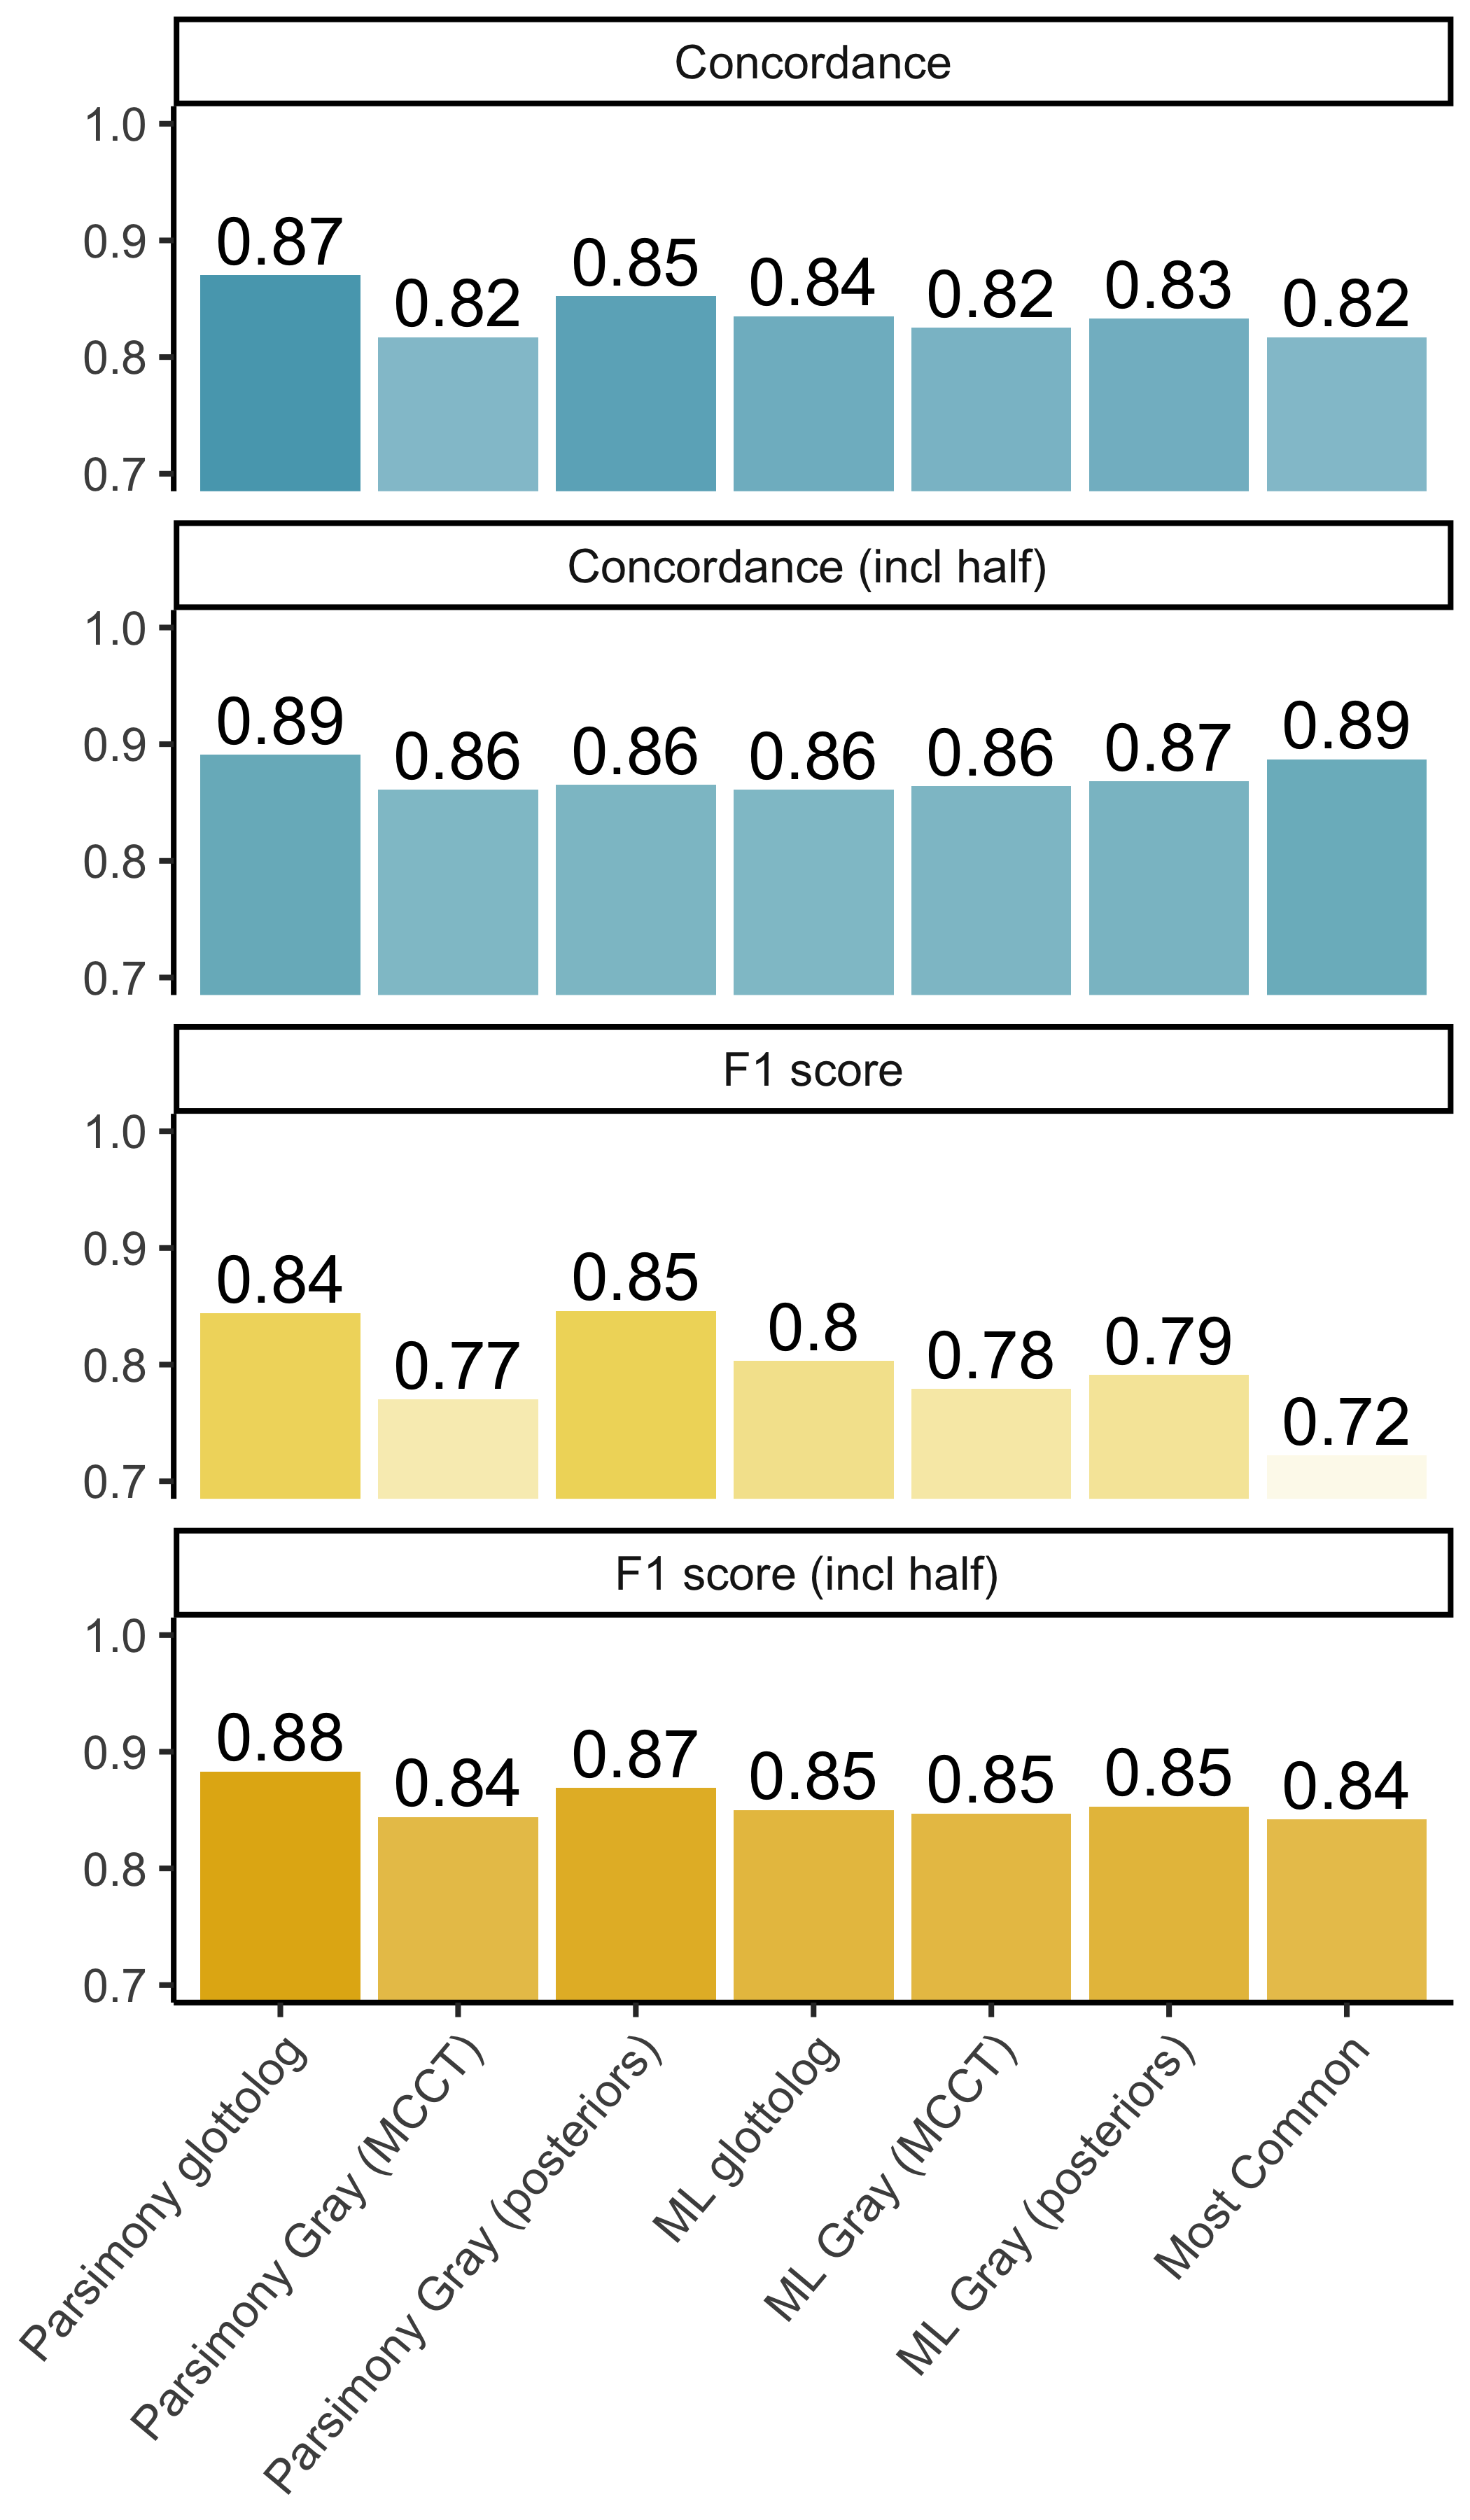
\includegraphics[width=11cm]{illustrations/plots_from_R/results/barplot_facet_scores.png}
\caption{\textbf{Barplots of concordance and F1-scores of each method.} NB that the y-axis starts from 0.7.}
\label{barplot_facet_results}
\end{figure}

The inclusion of the half-results have the effect of evening out the differences between the performance of the different methods. The concordance scores (including half-results) and the F1-scores (including half-results) for each method are more similar to each other.

Compared to the F1-scores from the lexical reconstruction of \citet{jager2018using}, all of the methods achieved higher scores. In this study, only statements about ancestral languages that could be mapped to Grambank-features were included. It is  possible that the study by \citet{jager2018using} had a greater overlap between all the reconstructions made by historical linguists and the meanings that they had data for. In that case, it is possible that the features that were possible to map to Grambank data were also those that Oceanic historical linguists are the most confident about --- hence the higher scores.

The method that tends to perform most similarly to historical linguists is Parsimony + the Glottolog 4.0 tree. The Glottolog 4.0 tree has a big disadvantage; it has no branch lengths and the topology is composed of a combination and compromise from several different sources as opposed to a principled and systematic investigation of lexical data. Parts of the tree are suggested by different scholars, which means that different clades are not necessarily comparable. It does have an advantage as well, and that is the sheer number of languages it includes. The overlap between languages included in \citet{grayetal_2009} is lower than the overlap between the Glottolog 4.0 tree and Grambank. It is possible that it is this sheer number of tips that gives it a greater concordance with historical linguists' predictions. The results also suggests that it is likely that historical linguists, in these specific studies, do not necessarily take into account branch lengths. 

Overall however, the methods preform similarly. Where they vary the most is for the plain F1-score (i.e. without including half-results). While it is appropriate to report this score as it is common practice when assessing performance in this manner, it is probably the score that is the least relevant for this particular study object since it entirely ignores True Negative-counts. Given that, if we focus instead on the concordance score there is very little that tells apart the different methods ---- they are giving very similar results. The results for MP and ML for the random 100 posterior samples performs slightly better than the plain MCC-tree, which may indicate that they are possibly picking up some relevant history not represented in the MCC-tree, such as horizontal transfer.

%As was discussed earlier, there are several different ways of evaluating the performance of these approaches. If we consider how often they made a prediction that agreed with historical linguistics out of all the times they made a confident prediction (Accuracy score excl Half/Half), then ML. If we award half a point for Half/Half predictions, Parsimony does better. However, in both instances the numbers are very close to each other.

%We are comparing our computational reconstruction results to those predicted by expert linguists. The reason that the Glottolog tree is more in line with the predictions from historical linguistics is probably because it resembles the tree most historical linguists are used to more than the Gray et al-2009 tree does (the Glottolog tree is based on \citet{blust_2009,blust_2014} and \citet{blust_chen_2017}). That is not to say it is necessarily a better reflection of the true history of these languages, but rather that it may fit better with the underlying model that the field of historical linguistics has been working with in recent decades. Most of the literature on reconstructions of Proto-Oceanic does not include detailed accounts of the exact tree topologies and branch lengths used to reconstruct the ancestral languages. As was shown in section \ref{sec:asr_methods}, we had to impute branch lengths for the Glottolog-tree. The manner by which reconstructions are postulated in historical linguistics is typically by considering how well distributed the phenomena are over certain genealogical and areal subgroups. If the distribution is convincingly non-random and the comparative method can be used to reconstruct forms, predictions about the proto-language are made (c.f. \citet[109-110]{pawley1973some}).

%Furthermore, there were fewer matches between languages for which there is Grambank data and the Gray et al Tree, making for more uncertainty in predicting ancestral states.

%In a similar study, \citet{jager2018using} attempt to reconstruct cognate classes for the proto-languages of three different language families. They used various approaches: binarising versus not binarising data; Maximum Parsimony versus Maximum Likelihood Estimation versus Minimal Lateral Networks; and using a single consensus tree versus sampling several from the tree posterior. The highest F1-score they achieved in this paper was 0.79 for the Maxmimum Likelihood Estimation reconstruction of Austronesian (using either a single tree or a sample of trees). This means that all of our results above perform ``better''. While this may be pleasing, it is not yet entirely clear why this is. 

%e were also somehow easier to reconstruct, and if so that would explain the higher F1-scores.
%\label{sec:ars:metod:hist}

%Many of the features that have been reconstructed for proto-languages of the Oceanic subgroup are also very common among Oceanic languages. For example, in our dataset 223 languages have a distinction between alienable and inalienable possession, and three do not have this feature . It is perhaps no surprise that historical linguists, Maximum Parsimony and Maximum Likelihood  agree that it is likely that the proto-languages have this feature as well\footnote{There was one exception. Maximum Likelihood on the Glottolog tree did not confidently predict presence of alienablity possession for Proto-Oceanic, the result was classified as ``half''. It did however predict alienablity for Proto-Polynesian.}. However, it is not always so simple. If this was all there was to it, we could just use raw distributions to reconstruct features of proto-languages. Historical linguists stress the importance of Maximum Parsimony and plausibility in their reconstructions, and as we saw in Fig. \ref{fig:clark_tree} (section \ref{sec:ars:metod:hist}), raw distributions alone can be misleading --- it is essential to take into account the tree structure. For example, \citet[118]{pawley1973some} suggests that verb-final word orders may have been possible in proto-Oceanic. This is tracked by feature GB133 \emph{`Is a pragmatically unmarked constituent order verb-final for transitive clauses?'}, and most languages are marked as `no' for this feature. However, Maximum Likelihood and the Gray et al 2009-tree did reconstruct presence of this feature at the root. 108 of the tips of this tree were absent, and 7 present, and yet the result was presence for Proto-Oceanic. This is (partially) due to the particular tree structure, where the languages with this feature attach further up in the tree structure (see Fig. \ref{GB133_tree_ML_gray})\footnote{It should be noted that the Maximum Parsimony result for the same tree did not reconstruct presence at the root. This has to do with the way Maximum Likelihood takes into account the distribution across the tree in each reconstruction, which gives the ancestral node of Maleu-Kilenge [male1289] and Kove [kove1237] a higher change of presence than it would under Maximum Parsimony.}\textsuperscript{,}\footnote{The languages with a presence for this feature are also mostly on the island of New Guinea and it is possible that this is a result of contact with non-Austronesian languages, as anonymous examiner 3 kindly pointed out.}.

%\newpage
%\begin{figure}
%\centering
%%%\includegraphics[width=\textwidth]{illustrations/plots_from_R/ML_gray_-GB133.png}
%\caption[Ancestral state reconstruction on tree for feature GB133, Gray et al 2009-tree and Maximum Likelihood.]{\textbf{Ancestral state reconstruction on tree for feature GB133, Gray et al 2009-tree and Maximum Likelihood. Yellow = presence, purple = absence.)}}
%\label{GB133_tree_ML_gray}
%\end{figure}
%

%
%It is often as revealing to study where the results got it ``wrong'' as where it was ``right''.Table~\ref{ASR_comparison_worst_table} shows the results for the automatic reconstructions that agreed the least with findings from classical historical linguistics. 
%
%%The two parsimony sets of results did propose that Proto-Oceanic did not have tense marking bound to the verb (GB082-GB084), nor is it by an inflecting word (GB121). However, when it came to tense marking by a particle and the aspect and mood marking, the automatic reconstructions were among the most dis-concordant with the expert predictions out of the entire dataset. In the Grambank dataset, we make a distinction between TAM-markers bound to the verb and free-standing markers that inflect versus those that don't. One possible factor that could have contributed to this is that TAM-markers in Oceanic languages are often described as forming portmanteau markers with subject markers. However, there is variation in how authors of grammars express this in their publications, and possibly also how our coders interpret the situation. This requires further investigation, which is unfortunately outside the scope of this study.

\subsection{New predictions}
Besides the predictions made by historical linguists, we can also explore what else has strong support in our computational reconstructions that is not explicitly mentioned in the literature. There are 110 features that are predicted as present in the four proto-languages by the two methods with each tree(s) (Glottolog, Gray et al 2009 MCCT and ditto posteriors); i.e. 6 times. For example, that Proto-Oceanic has inclusory constructions, Proto-Central Pacific uses verbs for property attribution (``adjectives'') and Proto-Polynesian has numeral classifiers.  A full list of these are found in Supplementary Material \ref{asr_table_extra}.

Many of these are probably not surprising to most historical linguists working on Oceanic languages, but they were not explicitly predicted in the sources surveyed for this study.

%three out of the four sets of results predicted that the order of numeral and noun is N-Num, all tests supported that ``adjectives'' in Proto-Central Pacific behaved like verbs when used predicatively, and all tests also supported that Proto-Polynesian had three or more distance contrasts among demonstratives. 

\subsection{Where the conflicts are: Ergativity}
The nature of the alignment system of Proto-Polynesian and Proto-Central Pacific is contested. \citet{clark1976aspects} posits, primarily on the basis of parsimony, that Proto-Polynesian was ergative whereas \citet{hale_1968}, \citet{hohepa_1967,hohepa_1969}, and \citet{chung1978} argue that it was accusative (while they suggest different historical pathways, they agree that Proto-Polynesian was nominative-accusative).

Grambank has two features that pertain to this argument:

\begin{itemize}
\item GB408 \emph{Is there any accusative alignment of flagging?}
\item GB409 \emph{Is there any ergative alignment of flagging?}
\end{itemize}

It is entirely possible for a language to be entered into the database as ``yes'' for several of these, i.e., from the perspective of Grambank languages aren't ``ergative'' or ``accusative'' --- they can have both ergative and accusative flagging simultaneously. This makes it possible for us to prove both Chung and Clark ``right'', the results can come out such that Proto-Polynesian had both accusative \emph{and} ergative alignment flagging. However, the results in fact come out strongly in favour of the proposal by Clark. Table \ref{conflict_results_table} shows that MP, ML and MC all reconstruct presence for ergative flagging in Proto-Polynesian. On the matter of nominative-accusative marking, there is disagreement with the MP results all suggesting absence but the ML and MC giving a half-result.

\newcommand{\pb}[1]{\parbox[t][][t]{1\linewidth}{#1} \vspace{3.5pt}}
% latex table generated in R 4.2.0 by xtable 1.8-4 package
% Tue Jul 19 16:54:44 2022
\begin{table}[ht]
\centering
\begin{tabular}{p{4cm}p{4cm}p{4cm}p{4cm}}
  \toprule
$\textbf{\parbox{1.8cm}{\raggedright Method}}$ & $\textbf{\pb{ GB408$\newline$Is there any accusative alignment of flagging?$\newline$Proto-Polynesian}}$ & $\textbf{\pb{ GB409$\newline$Is there any ergative alignment of flagging?$\newline$Proto-Polynesian}}$ & $\textbf{\pb{ GB409$\newline$Is there any ergative alignment of flagging?$\newline$Proto-Central Pacific}}$ \\ 
  \midrule
Parsimony Glottolog (v4.4) & Absent & Present & Absent \\ 
  Parsimony Gray et al (2009) - MCCT & Absent & Present & Absent \\ 
  Parsimony Gray et al (2009) - posteriors & Absent & Present & Absent \\ 
  ML Glottolog (v4.4) & Absent & Present & Absent \\ 
  ML Gray et al (2009) - MCCT & Half & Present & Absent \\ 
  ML Gray et al (2009) - posteriors & Half & Present & Absent \\ 
  Most Common & Half & Present & Present \\ 
   \bottomrule
\end{tabular}
\caption{Table showing the results for the features where historical linguists disagree.} 
\label{conflict_results_table}
\end{table}


As was noted earlier, the computational reconstructions differ from those arrived at through the comparative method primarily because the data used in this study is abstract presence or absence of structural features whereas historical linguists use specific concrete forms instead (c.f. \citet{crowley1985common}). In the case of alignment systems, the matter of concrete markers is less of an issue. However, besides the parsimony principle (as laid out by \citet[19]{clark1976aspects} for example), expert historical linguists also take into account the plausibility of the proposed proto-language and the chain of changes posited \citep{chung1977aspects}. It is not possible for the computational reconstructions to take these assumptions into account without having them formally described and introduced into the model, which is not possible at this time. This may be the reason for the lack of support for Chung's theory; the crucial information that underpins it is not accounted for in this study.

Given the topology of the trees used in this study, where the ergative flagging language Tongan is always attached to the Proto-Polynesian root at a higher level than Eastern Polynesian languages, it is very likely that GB409 would be reconstructed as present for Proto-Polynesian. As Clark pointed out, it is the most parsimonious solution. However, it could still have been the case that GB408 (accusative) would have been reconstructed for Proto-Polynesian. The reasons for this may lie in different definitions of what counts as nominative-accusative or neutral in different descriptions, and/or in discussions of plausibility. As has been discussed earlier, it was not possible to include plausibility as a factor in this study.

The proposals of \citet{hale_1968}, \citet{hohepa_1967, hohepa_1969}, and \citet{chung1978} also involve reconstruction of passive voice that relate to the development of the ergative systems. They suggest different pathways by which languages can develop from a nominative-accusative system to an ergative-absolutive one that rely on changes in the specifics of the passive voice construction that we unfortunately do not track. Given our data, which simply records presence of a productive passive voice marker on the verb, we are not able to scrutinise the three precise theories in greater detail. The results largely support the hypothesis that Proto-Eastern Polynesian had a passive voice marker and that Proto-Oceanic and Proto-Polynesian did not. This can be seen as partial support for the proposals by \citet{hale_1968, hohepa_1967, hohepa_1969, chung1978}.

Concerning the alignment of Proto-Central Pacific, all the results, save the Most Common-model, predict an absence of ergative-marking. This is likely to be because Rotuman [rotu1241], Wester Fijian [west2519] and Fijian [fiji1243] are all coded as 0 for this feature and they split of early from the Proto-Central Pacific node. This supports the argument put forward by \citet{ball2007ergativity}. Similarity to the Polynesian case, given the tree structure it is difficult for the computational approaches to produce another result in lieu of more information on the particulars of the development of alignment systems or possible horizontal transfer.

\section{Conclusions}
In this paper, we have investigated the history of structural features of Oceanic languages to examine how computational reconstructive methods compare to reconstructions by historical linguists, including contributing to the debate on  alignment in Oceanic proto-languages.

We have found that computational reconstructions show a high degree of concordance with reconstructions from expert historical linguists. Reconstructions by both Maximum Parsimony and Maximum Likelihood agreed to a very large extent with the findings from historical linguistics. This suggests that the mechanisms at work in historical linguistic reconstruction are similar to the computational methods presented in this paper. This means that we have support for using conclusions regarding rate of change etc from the computational methods to estimate knowledge of historical linguists. This can aid us in making the implicit explicit. Whether or not the predictions from classical historical linguistics are correct or not is a different matter, which should be investigated by assessing the soundness of the principles at play and comparing with other evidence.

The future of research on the history of languages probably lies in the combination of human and computational labour. Computational endeavours of curating lexical cognate data \citep{list2022lexibank} and constructing trees \citep{grayetal_2009} still rely on teams of expert linguists annotating wordlists for cognacy. Methods are being developed for automatic cognate detection \citep{list2017potential}, but they are not yet ready to replace the vast human knowledge and experience of the experts of historical linguistics. However, once cognate classes, regular sound correspondences and structural features are identified the work then turns to subgrouping (constructing trees/networks) and reconstructing earlier states. For these tasks, there are suitable computational methods that can be applied. These tasks can be greatly improved and effectivized by computational tools.

In order to improve these methods, we could attempt to include the knowledge that historical linguists have about plausibility of changes, harmonics of traits and contact events. This kind of information can be incorporated to guide computational methods, but should not be given the power to entirely constrain them. In order for this to happen, more information needs to be made explicit in historical linguistics studies.

The more information is made explicit in methodology the easier it is to assess the soundness of the study, replicate it and improve upon it. This study aims at increasing the transparency of both the principles of reconstruction in classical historical linguistics and the corresponding  computational approaches. Hopefully this study (alongside \citet{carling2021} and \citet{goldstein_2022}) can be a starting point for more joint ventures into our grammatical past.

%In addition, we also need to encourage co-operation between traditional historical linguists and linguists applying new methods, as exemplified in this paper, when it comes to estimating branch lengths. Many trees proposed in classical studies of historical linguistics do not necessarily 

%One of the key pieces of information that is missing from this analysis is plausibility of changes and combinations of features.

%Within Oceanic historical linguistics, there exists a debate regarding the nature of the alignment system of Proto-Polynesian. The results of this study support the analysis that it was ergative. However, since the computational reconstructions are unable to take into account considerations of plausibility, which is the main difference between the different proposals, this cannot be taken as hard evidence. Further work in this area should seek to incorporate information about plausibility in order to increase the reliability of this result.

%explicit information on plausibility of rate of change and combinations of traits
%ways of estimating contact events
%models of history (trees/networks) with meaningful branch/edge lengths
%more training of computational methods to historical linguistics students
%more carefully coded data from HL to input to reasonable computational models


\newpage

\singlespacing
\bibliographystyle{Hedvig_bibtex_style_PhD}
\bibliography{HS_ASR}
%\singlespacing


\newpage
\singlespacing
\appendix
\section*{Appendices}
\addcontentsline{toc}{section}{Appendices}
\renewcommand{\thesubsection}{\Alph{subsection}}

\subsection{Data availability}
\label{supp:data_avail}
The Grambank-dataset (version 1.0) will be published shortly and can be provided for anonymous reviewers under the condition that it is not shared before official publication. All code relevant to this paper will be published as a Git repository and how-ever the journal might want it published. The Git repository is private and is possible for reviewers to access under certain restrictions before publication.

\subsection{Technical details of methods}
\label{supp:tech_details}

For Maximum Parsimony, we are using the function \texttt{asr\_max\_parsimony()} from the R-package \texttt{castor} \citep{louca2017efficient} (which is an instantiation of the method described in \citet{sankoff1975minimal}) for calculating ancestral states and stability of features. This function produces ancestral states for all nodes and reports the number of changes that was minimally required for each feature. 

Ancestral state reconstruction using Maximum Likelihood Estimation involves computing each ancestral state from the tips up to the root taking into account branch lengths and the joint likelihood of states given all nodes in the tree \citep{wilks1938large, fisher1912absolute, pagel1994detecting, cunningham1998reconstructing}. The Maximum Likelihood Estimation function takes a set of observations and computes the parameter distribution that maximises the likelihood given the observed data\footnote{For a gentle introduction to the concept of Maximum Likelihood Estimation, see \citet{jonny_ML}.}. This means that for every split in the tree --- every ancestral node --- the Maximum Likelihood Estimation function computes what is the most likely distribution at that point given the nature of the entire tree. ML can be modified so that it allows for different rates of change. An Equal Rates (ER) model assumes that the chance of transition from state A to state B and from B to A are equal. However, we as linguists are aware that certain features are more likely to be lost than gained so this is not a reasonable assumption. Therefore, we allow the model to estimate different transition rates for going from A to B and from B to A given the data. This is known as ``All Rates are Different'' (ARD).

When estimating ancestral states with ML, it is possible to either a) find the state at each node that maximises the likelihood (integrating over all other states at all nodes, in proportion to their probability) at that particular node (marginal reconstruction), or b) find the set of character states at all nodes that (jointly) maximize the likelihood of the entire tree (joint reconstruction). We are using marginal reconstruction in this study since it is the recommended way to deal with uncertainty in reconstruction \citep{revell_2014}. These two methods often yield similar results, but can differ, see \citet[259-260]{felsenstein2004inferring},  \citet[121-126]{yang2006computational} and \citet[5]{joy2016ancestral} for more details. For our data, a trial run of joint reconstruction did not generate drastically different outcomes.

For this study, the function \texttt{corHMM} from the \texttt{R}-package \texttt{corHMM} \citep{corHMM} is used for marginal reconstruction of ancestral states and rates of change per feature. %Missing data in Grambank for languages included in the analysis was converted to ambiguous, (i.e ? in Grambank $\rightarrow$ 0\&1 for rayDISC()). 

For the analysis of conservatism per language, the function \texttt{optim.pml()} from \texttt{Phangorn} \citep{phangorn} was used. This function rescales the branches in accordance with the Maximum Likelihood Estimation of change along them. The process of re-scaling the tree in this manner unroots the tree; instead of having root, branches and tips, it becomes an acyclic graph of tips connected by lines of appropriate length. Unrooted trees can be re-rooted using midpoting rooting, outgroup rooting or other methods\footnote{For a visual introduction to outgroup rooting, see \href{this blogpost}{https://phylobotanist.blogspot.com/2015/01/how-to-root-phylogenetic-tree-outgroup.html} by PhyloBotanist.}. For this study, the trees were re-rooted using Nanggu [nang1262], Ayiwoo [ayiw1239] or Natügu [natu1246] as an outgroup. As with the Maximum Parsimony analysis, the distance from the root to each tip was carried out with \texttt{distTip} and the distances were rescaled to between 0 and 1. 

Languages with missing data were pruned away in all analysis, no hidden state reconstruction of values at tips was preformed. Because Nanggu, Ayiwoo and Natügu was used as an outgroup to root the trees in the conservatism analysis, features which these three languages lacked were excluded from the conservatism analysis. This left 167 Grambank features which were included in the conservatism analysis. %#update

Concerning missing data generally, for both methods the trees from Glottolog and \citet{grayetal_2009} were pruned to only tips representing Oceanic languages which are also found in Grambank. The match between Glottolog and Grambank is 226, the match between \citet{grayetal_2009} and Grambank is 112. For the parsimony analysis of each feature, languages with missing data were dropped from the trees in the analysis for that feature. Features which could only be assigned values for less than half of the languages in the tree were excluded from the analysis.

For both Maximum Parsimony and Maximum Likelihood it is possible for a structural feature to appear and disappear several times along a lineage. This is different from cognate data where a cognate class cannot re-appear.

\subsection{Mathematics of the F1-score including half-results}
\label{math_supp}

I am very grateful for the assistance of Stephen Mann in working out the mathematics of these scores as they incorporate the Half-results.

\subsubsection{Standard definitions}\label{sec:standard}

The F1-score is the harmonic mean of precision and recall \citep{van1979information}.

\begin{align*}
    F_1 &= 2\times\frac{\text{precision}\times\text{recall}}
            {\text{precision} + \text{recall}}\\
        &= \frac{\text{TP}}
            {\text{TP}+\frac{1}{2}\times(\text{FP}+\text{FN})}
\end{align*}

\begin{align*}
    \text{precision} 
        &= \frac{\text{TP}}
            {\text{TP}+\text{FP}}
\end{align*}

\begin{align*}
    \text{recall} 
        &= \frac{\text{TP}}
            {\text{TP}+\text{FN}}
\end{align*}

%%%%%%%%%%%
%%%%%%%%%%%
%%%%%%%%%%%
%%%%%%%%%%%
\subsubsection{Half-result definitions of precision and recall}\label{sec:halfsies}

The half-result-definitions of precision and recall add one half of the half-counts to the numerator, and all of the half-counts to the denominator:

\begin{equation*}
    \text{precision}_{\text{half}} 
        = \frac{\text{TP}+\frac{\text{H}}{2}}
            {\text{TP}+\text{FP}+\text{H}}
\end{equation*}

\begin{equation*}
    \text{recall}_{\text{half}}
        = \frac{\text{TP}+\frac{\text{H}}{2}}
            {\text{TP}+\text{FN}+\text{H}}
\end{equation*}

%%%%%%%%%%%
%%%%%%%%%%%
%%%%%%%%%%%
%%%%%%%%%%%
\subsubsection{The question}\label{sec:question}

We want to define $F_{1,\text{half}}$.
A natural way to do it would be to follow the rule defined above, i.e.

\begin{equation*}
    F_{1,\text{half?}} = \frac{\text{TP}+\frac{\text{H}}{2}}
            {\text{TP}+\frac{1}{2}\times(\text{FP}+\text{FN}) + \text{H}}
\end{equation*}

\noindent However, we want to ensure $F_{1,\text{half}}$ has the same relationship with $\text{precision}_{\text{half}}$ and $\text{recall}_{\text{half}}$ as $F_1$ has with precision and recall.
So we need to determine whether the following equation is true:

\begin{equation}\label{eq:question}
    2\times\frac{\text{precision}_{\text{half}}\times\text{recall}_{\text{half}}}
            {\text{precision}_{\text{half}} + \text{recall}_{\text{half}}}
    \stackrel{?}{=}
    \frac{\text{TP}+\frac{\text{H}}{2}}
            {\text{TP}+\frac{1}{2}\times(\text{FP}+\text{FN}) + \text{H}}
\end{equation}

%%%%%%%%%%%
%%%%%%%%%%%
%%%%%%%%%%%
%%%%%%%%%%%
\subsubsection{The proof}\label{sec:proof}

We will expand the left-hand side of \eqref{eq:question} and show it is equal to the right-hand side.
Let's forget about the $2\times$ for now (we will reintroduce it at the end).
Expanding the numerator gives:

\begin{equation*}
    \frac{\left(
        \text{TP}+\frac{\text{H}}{2}
    \right)\left(
        \text{TP}+\frac{\text{H}}{2}
    \right)}
    {\left(
        \text{TP} + \text{FP} + \text{H}
    \right)\left(
        \text{TP} + \text{FN} + \text{H}
    \right)}
\end{equation*}

\noindent Expanding the denominator gives:

\begin{align*}
    &\frac{\text{TP}+\frac{\text{H}}{2}}
    {\text{TP}+\text{FP}+\text{H}}
    +
    \frac{\text{TP}+\frac{\text{H}}{2}}
    {\text{TP}+\text{FN}+\text{H}}\\[1.5ex]
    &=
    %% Second line, left part
    %% Numerator
    \frac{\left(
        \text{TP}+\frac{\text{H}}{2}
    \right)\left(
        \text{TP}+\text{FN}+\text{H}
    \right)}
    %% Denominator
    {\left(
        \text{TP}+\text{FP}+\text{H}
    \right)\left(
        \text{TP}+\text{FN}+\text{H}
    \right)}
    +
    %% Second line, right part
    %% Numerator
    \frac{\left(
        \text{TP}+\frac{\text{H}}{2}
    \right)\left(
        \text{TP}+\text{FP}+\text{H}
    \right)}
    %% Denominator
    {\left(
        \text{TP}+\text{FN}+\text{H}
    \right)\left(
        \text{TP}+\text{FP}+\text{H}
    \right)}\\[1.5ex]
    %% Third line
    &=\frac{\left(
        \text{TP}+\frac{\text{H}}{2}
    \right)\left(
        2\times\text{TP} + \text{FP} + \text{FN} + 2\times\text{H}
    \right)}
    {\left(
        \text{TP}+\text{FP}+\text{H}
    \right)\left(
        \text{TP}+\text{FN}+\text{H}
    \right)}
\end{align*}

\noindent When we put the numerator back on top of the denominator, both of their respective denominators cancel out, because they are both $(\text{TP}+\text{FP}+\text{H})(\text{TP}+\text{FN}+\text{H})$.
So we end up with \emph{the numerator of the numerator} on top of \emph{the numerator of the denominator}, like so:

\begin{align*}
    &\frac{\left(
        \text{TP}+\frac{\text{H}}{2}
    \right)\left(
        \text{TP}+\frac{\text{H}}{2}
    \right)}
    {\left(
        \text{TP}+\frac{\text{H}}{2}
    \right)\left(
        2\times\text{TP} + \text{FP} + \text{FN} + 2\times\text{H}
    \right)}\\[1.5ex]
    &=
    \frac{\left(
        \text{TP}+\frac{\text{H}}{2}
    \right)}
    {2\times\text{TP} + \text{FP} + \text{FN} + 2\times\text{H}}
\end{align*}

\noindent Finally, we bring back the $2\times$ from the beginning:

\begin{align*}
    &2\times\frac{\left(
        \text{TP}+\frac{\text{H}}{2}
    \right)}
    {2\times\text{TP} + \text{FP} + \text{FN} + 2\times\text{H}}\\[1ex]
    &=
    \frac{\text{TP}+\frac{\text{H}}{2}}
    {\text{TP} + \frac{1}{2}\times(\text{FP} + \text{FN}) + \text{H}}
\end{align*}

\noindent And we have our suggested definition of $F_{1,\text{half}}$ as required.

\subsection{Binarisation of the Grambank features}
\label{supp:dataset_details}
Most of the feature questions are binary (GB027: Are nominal conjunction and comitative expressed by different elements?) but a few are multi-state (GB024 What is the order of numeral and noun in the NP? 1) Num-N, 2) N-Num, 3) both). For the analysis in this study, the multi-state features have been binarised. This is because the values of the multi-state features are not independent of each other; they all contain the value ``Both''. The value ``Num-N'' (numeral before noun) of GB024 is more similar to ``Both'' than it is to the other alternative ``N-Num''. The relationship between the three values are not equal or independent. The table in \ref{Grambank_features} contains a list of all the features used in this study, including the binarised features. The binarization results in a total of 201 features. 

\newpage
\subsection{Grambank features}
\label{Grambank_features}

\singlespacing
\begin{landscape}
% latex table generated in R 4.3.0 by xtable 1.8-4 package
% Sat Jun 10 22:23:05 2023
\begin{longtable}{p{3cm}p{12cm}}
  \toprule
Feature_ID & Name \\ 
  \midrule
GB024a & Is the order of the numeral and noun Num-N? \\ 
  GB024b & Is the order of the numeral and noun N-Num? \\ 
  GB025a & Is the order of the adnominal demonstrative and noun Dem-N? \\ 
  GB025b & Is the order of the adnominal demonstrative and noun N-Dem? \\ 
  GB065a & Is the pragmatically unmarked order of adnominal possessor noun and possessed noun PSR-PSD? \\ 
  GB065b & Is the pragmatically unmarked order of adnominal possessor noun and possessed noun PSD-PSR? \\ 
  GB130a & Is the pragmatically unmarked order of S and V in intransitive clauses S-V? \\ 
  GB130b & Is the pragmatically unmarked order of S and V in intransitive clauses V-S? \\ 
  GB193a & Is the order of the adnominal property word (ANM) and noun ANM-N? \\ 
  GB193b & Is the order of the adnominal property word (ANM) and noun N-ANM? \\ 
  GB203a & Is the order of the adnominal collective universal quantifier (UQ) and noun UQ-N? \\ 
  GB203b & Is the order of the adnominal collective universal quantifier (UQ) and noun N-QU? \\ 
  GB020 & Are there definite or specific articles? \\ 
  GB021 & Do indefinite nominals commonly have indefinite articles? \\ 
  GB022 & Are there prenominal articles? \\ 
  GB023 & Are there postnominal articles? \\ 
  GB026 & Can adnominal property words occur discontinuously? \\ 
  GB027 & Are nominal conjunction and comitative expressed by different elements? \\ 
  GB028 & Is there a distinction between inclusive and exclusive? \\ 
  GB030 & Is there a gender distinction in independent 3rd person pronouns? \\ 
  GB031 & Is there a dual or unit augmented form (in addition to plural or augmented) for all person categories in the pronoun system? \\ 
  GB035 & Are there three or more distance contrasts in demonstratives? \\ 
  GB036 & Do demonstratives show an elevation distinction? \\ 
  GB037 & Do demonstratives show a visible-nonvisible distinction? \\ 
  GB038 & Are there demonstrative classifiers? \\ 
  GB039 & Is there nonphonological allomorphy of noun number markers? \\ 
  GB041 & Are there several nouns (more than three) which are suppletive for number? \\ 
  GB042 & Is there productive overt morphological singular marking on nouns? \\ 
  GB043 & Is there productive morphological dual marking on nouns? \\ 
  GB044 & Is there productive morphological plural marking on nouns? \\ 
  GB046 & Is there an associative plural marker for nouns? \\ 
  GB047 & Is there a productive morphological pattern for deriving an action/state noun from a verb? \\ 
  GB048 & Is there a productive morphological pattern for deriving an agent noun from a verb? \\ 
  GB049 & Is there a productive morphological pattern for deriving an object noun from a verb? \\ 
  GB051 & Is there a gender/noun class system where sex is a factor in class assignment? \\ 
  GB052 & Is there a gender/noun class system where shape is a factor in class assignment? \\ 
  GB053 & Is there a gender/noun class system where animacy is a factor in class assignment? \\ 
  GB054 & Is there a gender/noun class system where plant status is a factor in class assignment? \\ 
  GB057 & Are there numeral classifiers? \\ 
  GB058 & Are there possessive classifiers? \\ 
  GB059 & Is the adnominal possessive construction different for alienable and inalienable nouns? \\ 
  GB068 & Do core adjectives (defined semantically as property concepts such as value, shape, age, dimension) act like verbs in predicative position? \\ 
  GB069 & Do core adjectives (defined semantically as property concepts; value, shape, age, dimension) used attributively require the same morphological treatment as verbs? \\ 
  GB070 & Are there morphological cases for non-pronominal core arguments (i.e. S/A/P)? \\ 
  GB071 & Are there morphological cases for pronominal core arguments (i.e. S/A/P)? \\ 
  GB072 & Are there morphological cases for oblique non-pronominal NPs (i.e. not S/A/P)? \\ 
  GB073 & Are there morphological cases for independent oblique personal pronominal arguments (i.e. not S/A/P)? \\ 
  GB074 & Are there prepositions? \\ 
  GB075 & Are there postpositions? \\ 
  GB079 & Do verbs have prefixes/proclitics, other than those that only mark A, S or P (do include portmanteau: A \& S + TAM)? \\ 
  GB080 & Do verbs have suffixes/enclitics, other than those that only mark A, S or P (do include portmanteau: A \& S + TAM)? \\ 
  GB081 & Is there productive infixation in verbs? \\ 
  GB082 & Is there overt morphological marking of present tense on verbs? \\ 
  GB083 & Is there overt morphological marking on the verb dedicated to past tense? \\ 
  GB084 & Is there overt morphological marking on the verb dedicated to future tense? \\ 
  GB086 & Is a morphological distinction between perfective and imperfective aspect available on verbs? \\ 
  GB089 & Can the S argument be indexed by a suffix/enclitic on the verb in the simple main clause? \\ 
  GB090 & Can the S argument be indexed by a prefix/proclitic on the verb in the simple main clause? \\ 
  GB091 & Can the A argument be indexed by a suffix/enclitic on the verb in the simple main clause? \\ 
  GB092 & Can the A argument be indexed by a prefix/proclitic on the verb in the simple main clause? \\ 
  GB093 & Can the P argument be indexed by a suffix/enclitic on the verb in the simple main clause? \\ 
  GB094 & Can the P argument be indexed by a prefix/proclitic on the verb in the simple main clause? \\ 
  GB095 & Are variations in marking strategies of core participants based on TAM distinctions? \\ 
  GB096 & Are variations in marking strategies of core participants based on verb classes? \\ 
  GB098 & Are variations in marking strategies of core participants based on person distinctions? \\ 
  GB099 & Can verb stems alter according to the person of a core participant? \\ 
  GB103 & Is there a benefactive applicative marker on the verb (including indexing)? \\ 
  GB104 & Is there an instrumental applicative marker on the verb (including indexing)? \\ 
  GB105 & Can the recipient in a ditransitive construction be marked like the monotransitive patient? \\ 
  GB107 & Can standard negation be marked by an affix, clitic or modification of the verb? \\ 
  GB108 & Is there directional or locative morphological marking on verbs? \\ 
  GB109 & Is there verb suppletion for participant number? \\ 
  GB110 & Is there verb suppletion for tense or aspect? \\ 
  GB111 & Are there conjugation classes? \\ 
  GB113 & Are there verbal affixes or clitics that turn intransitive verbs into transitive ones? \\ 
  GB114 & Is there a phonologically bound reflexive marker on the verb? \\ 
  GB115 & Is there a phonologically bound reciprocal marker on the verb? \\ 
  GB116 & Do verbs classify the shape, size or consistency of absolutive arguments by means of incorporated nouns, verbal affixes or suppletive verb stems? \\ 
  GB117 & Is there a copula for predicate nominals? \\ 
  GB118 & Are there serial verb constructions? \\ 
  GB119 & Can mood be marked by an inflecting word (""""""""auxiliary verb"""""""")? \\ 
  GB120 & Can aspect be marked by an inflecting word (""""""""auxiliary verb"""""""")? \\ 
  GB121 & Can tense be marked by an inflecting word (""""""""auxiliary verb"""""""")? \\ 
  GB122 & Is verb compounding a regular process? \\ 
  GB123 & Are there verb-adjunct (aka light-verb) constructions? \\ 
  GB124 & Is incorporation of nouns into verbs a productive intransitivizing process? \\ 
  GB126 & Is there an existential verb? \\ 
  GB127 & Are different posture verbs used obligatorily depending on an inanimate locatum's shape or position (e.g. 'to lie' vs. 'to stand')? \\ 
  GB129 & Is there a notably small number, i.e. about 100 or less, of verb roots in the language? \\ 
  GB131 & Is a pragmatically unmarked constituent order verb-initial for transitive clauses? \\ 
  GB132 & Is a pragmatically unmarked constituent order verb-medial for transitive clauses? \\ 
  GB133 & Is a pragmatically unmarked constituent order verb-final for transitive clauses? \\ 
  GB134 & Is the order of constituents the same in main and subordinate clauses? \\ 
  GB135 & Do clausal objects usually occur in the same position as nominal objects? \\ 
  GB136 & Is the order of core argument (i.e. S/A/P) constituents fixed? \\ 
  GB137 & Can standard negation be marked clause-finally? \\ 
  GB138 & Can standard negation be marked clause-initially? \\ 
  GB139 & Is there a difference between imperative (prohibitive) and declarative negation constructions? \\ 
  GB140 & Is verbal predication marked by the same negator as all of the following types of predication: locational, existential and nominal? \\ 
  GB146 & Is there a morpho-syntactic distinction between predicates expressing controlled versus uncontrolled events or states? \\ 
  GB147 & Is there a morphological passive marked on the lexical verb? \\ 
  GB148 & Is there a morphological antipassive marked on the lexical verb? \\ 
  GB149 & Is there a morphologically marked inverse on verbs? \\ 
  GB150 & Is there clause chaining? \\ 
  GB151 & Is there an overt verb marker dedicated to signalling coreference or noncoreference between the subject of one clause and an argument of an adjacent clause (""""""""switch reference"""""""")? \\ 
  GB152 & Is there a morphologically marked distinction between simultaneous and sequential clauses? \\ 
  GB155 & Are causatives formed by affixes or clitics on verbs? \\ 
  GB156 & Is there a causative construction involving an element that is unmistakably grammaticalized from a verb for 'to say'? \\ 
  GB158 & Are verbs reduplicated? \\ 
  GB159 & Are nouns reduplicated? \\ 
  GB160 & Are elements apart from verbs or nouns reduplicated? \\ 
  GB165 & Is there productive morphological trial marking on nouns? \\ 
  GB166 & Is there productive morphological paucal marking on nouns? \\ 
  GB167 & Is there a logophoric pronoun? \\ 
  GB170 & Can an adnominal property word agree with the noun in gender/noun class? \\ 
  GB171 & Can an adnominal demonstrative agree with the noun in gender/noun class? \\ 
  GB172 & Can an article agree with the noun in gender/noun class? \\ 
  GB177 & Can the verb carry a marker of animacy of argument, unrelated to any gender/noun class of the argument visible in the NP domain? \\ 
  GB184 & Can an adnominal property word agree with the noun in number? \\ 
  GB185 & Can an adnominal demonstrative agree with the noun in number? \\ 
  GB186 & Can an article agree with the noun in number? \\ 
  GB187 & Is there any productive diminutive marking on the noun (exclude marking by system of nominal classification only)? \\ 
  GB188 & Is there any productive augmentative marking on the noun (exclude marking by system of nominal classification only)? \\ 
  GB192 & Is there a gender system where a noun's phonological properties are a factor in class assignment? \\ 
  GB196 & Is there a male/female distinction in 2nd person independent pronouns? \\ 
  GB197 & Is there a male/female distinction in 1st person independent pronouns? \\ 
  GB198 & Can an adnominal numeral agree with the noun in gender/noun class? \\ 
  GB204 & Do collective ('all') and distributive ('every') universal quantifiers differ in their forms or their syntactic positions? \\ 
  GB250 & Can predicative possession be expressed with a transitive 'habeo' verb? \\ 
  GB252 & Can predicative possession be expressed with an S-like possessum and a locative-coded possessor? \\ 
  GB253 & Can predicative possession be expressed with an S-like possessum and a dative-coded possessor? \\ 
  GB254 & Can predicative possession be expressed with an S-like possessum and a possessor that is coded like an adnominal possessor? \\ 
  GB256 & Can predicative possession be expressed with an S-like possessor and a possessum that is coded like a comitative argument? \\ 
  GB257 & Can polar interrogation be marked by intonation only? \\ 
  GB260 & Can polar interrogation be indicated by a special word order? \\ 
  GB262 & Is there a clause-initial polar interrogative particle? \\ 
  GB263 & Is there a clause-final polar interrogative particle? \\ 
  GB264 & Is there a polar interrogative particle that most commonly occurs neither clause-initially nor clause-finally? \\ 
  GB265 & Is there a comparative construction that includes a form that elsewhere means 'surpass, exceed'? \\ 
  GB266 & Is there a comparative construction that employs a marker of the standard which elsewhere has a locational meaning? \\ 
  GB270 & Can comparatives be expressed using two conjoined clauses? \\ 
  GB273 & Is there a comparative construction with a standard marker that elsewhere has neither a locational meaning nor a 'surpass/exceed' meaning? \\ 
  GB275 & Is there a bound comparative degree marker on the property word in a comparative construction? \\ 
  GB276 & Is there a non-bound comparative degree marker modifying the property word in a comparative construction? \\ 
  GB285 & Can polar interrogation be marked by a question particle and verbal morphology? \\ 
  GB286 & Can polar interrogation be indicated by overt verbal morphology only? \\ 
  GB291 & Can polar interrogation be marked by tone? \\ 
  GB296 & Is there a phonologically or morphosyntactically definable class of ideophones that includes ideophones depicting imagery beyond sound? \\ 
  GB297 & Can polar interrogation be indicated by a V-not-V construction? \\ 
  GB298 & Can standard negation be marked by an inflecting word (""""""""auxiliary verb"""""""")? \\ 
  GB299 & Can standard negation be marked by a non-inflecting word (""""""""auxiliary particle"""""""")? \\ 
  GB300 & Does the verb for 'give' have suppletive verb forms? \\ 
  GB301 & Is there an inclusory construction? \\ 
  GB302 & Is there a phonologically free passive marker (""""""""particle"""""""" or """"""""auxiliary"""""""")? \\ 
  GB303 & Is there a phonologically free antipassive marker (""""""""particle"""""""" or """"""""auxiliary"""""""")? \\ 
  GB304 & Can the agent be expressed overtly in a passive clause? \\ 
  GB305 & Is there a phonologically independent reflexive pronoun? \\ 
  GB306 & Is there a phonologically independent non-bipartite reciprocal pronoun? \\ 
  GB309 & Are there multiple past or multiple future tenses, distinguishing distance from Time of Reference? \\ 
  GB312 & Is there overt morphological marking on the verb dedicated to mood? \\ 
  GB313 & Are there special adnominal possessive pronouns that are not formed by an otherwise regular process? \\ 
  GB314 & Can augmentative meaning be expressed productively by a shift of gender/noun class? \\ 
  GB315 & Can diminutive meaning be expressed productively by a shift of gender/noun class? \\ 
  GB316 & Is singular number regularly marked in the noun phrase by a dedicated phonologically free element? \\ 
  GB317 & Is dual number regularly marked in the noun phrase by a dedicated phonologically free element? \\ 
  GB318 & Is plural number regularly marked in the noun phrase by a dedicated phonologically free element? \\ 
  GB319 & Is trial number regularly marked in the noun phrase by a dedicated phonologically free element? \\ 
  GB320 & Is paucal number regularly marked in the noun phrase by a dedicated phonologically free element? \\ 
  GB321 & Is there a large class of nouns whose gender/noun class is not phonologically or semantically predictable? \\ 
  GB322 & Is there grammatical marking of direct evidence (perceived with the senses)? \\ 
  GB323 & Is there grammatical marking of indirect evidence (hearsay, inference, etc.)? \\ 
  GB324 & Is there an interrogative verb for content interrogatives (who?, what?, etc.)? \\ 
  GB325 & Is there a count/mass distinction in interrogative quantifiers? \\ 
  GB326 & Do (nominal) content interrogatives normally or frequently occur in situ? \\ 
  GB327 & Can the relative clause follow the noun? \\ 
  GB328 & Can the relative clause precede the noun? \\ 
  GB329 & Are there internally-headed relative clauses? \\ 
  GB330 & Are there correlative relative clauses? \\ 
  GB331 & Are there non-adjacent relative clauses? \\ 
  GB333 & Is there a decimal numeral system? \\ 
  GB334 & Is there synchronic evidence for any element of a quinary numeral system? \\ 
  GB335 & Is there synchronic evidence for any element of a vigesimal numeral system? \\ 
  GB336 & Is there a body-part tallying system? \\ 
  GB400 & Are all person categories neutralized in some voice, tense, aspect, mood and/or negation? \\ 
  GB401 & Is there a class of patient-labile verbs? \\ 
  GB402 & Does the verb for 'see' have suppletive verb forms? \\ 
  GB403 & Does the verb for 'come' have suppletive verb forms? \\ 
  GB408 & Is there any accusative alignment of flagging? \\ 
  GB409 & Is there any ergative alignment of flagging? \\ 
  GB410 & Is there any neutral alignment of flagging? \\ 
  GB415 & Is there a politeness distinction in 2nd person forms? \\ 
  GB421 & Is there a preposed complementizer in complements of verbs of thinking and/or knowing? \\ 
  GB422 & Is there a postposed complementizer in complements of verbs of thinking and/or knowing? \\ 
  GB430 & Can adnominal possession be marked by a prefix on the possessor? \\ 
  GB431 & Can adnominal possession be marked by a prefix on the possessed noun? \\ 
  GB432 & Can adnominal possession be marked by a suffix on the possessor? \\ 
  GB433 & Can adnominal possession be marked by a suffix on the possessed noun? \\ 
  GB519 & Can mood be marked by a non-inflecting word (""""""""auxiliary particle"""""""")? \\ 
  GB520 & Can aspect be marked by a non-inflecting word (""""""""auxiliary particle"""""""")? \\ 
  GB521 & Can tense be marked by a non-inflecting word (""""""""auxiliary particle"""""""")? \\ 
  GB522 & Can the S or A argument be omitted from a pragmatically unmarked clause when the referent is inferrable from context (""""""""pro-drop"""""""" or """"""""null anaphora"""""""")? \\ 
   \bottomrule
\caption{Table of Grambank fetures} 
\label{GB_features_table}
\end{longtable}

\end{landscape}
\newpage


\subsection{Further details on the tree phylogeny}
\label{supp:tree_details}

The tree from \citet{grayetal_2009} contains duplicates (see for example Nakanai). This is because it is a tree of word-lists for languages (doculects) rather than languages themselves. There are also some instances where multiple dialects of one language is included. For the analysis, only one tip per language was retained, based on which had best coverage in the underlying data for the tree (i.e. the Austronesian Basic Vocabulary Database, ABVD \citep{ABVD}). This means that duplicate languages were reduced to one, and only one dialect per language retained if there was more than one. 

For both Maximum Parsimony and Maximum Likelihood the tree were first pruned down to only languages where there is data in Grambank. For the further Maximum Parsimony analysis, tips representing languages where the data for a particular feature was missing were dropped for the analysis of that feature. For the Maximum Likelihood analysis, the value at such tips was converted to ambiguous. This is necessary because otherwise the rate of change across the different features would not be comparable in the Maximum Likelihood analysis.

\subsection{Further details on the Grambank coding of proto-languages }
\label{supp:proto_lg_coding}
Another example of how information in the publications was turned into Grambank feature coding relates to verbal markers encoding subjects and objects, as proposed by \citet{lynchrosscrowley_proto_grammar_oceanic} among others. In their book, there is a paper on reconstructions of grammar for Proto-Oceanic and in the section on the basic verb phrase we find the statement below:

\begin{quotation}
\noindent\emph{Attached to the verb root were a subject proclitic and, if the verb had a non-generic object, an object enclitic.} \end{quotation} \begin{flushright} \citet[83]{lynchrosscrowley_proto_grammar_oceanic} \end{flushright}

This statement, together with a verb schema provided in the section, support the notion that Proto-Oceanic had subject proclitics and object enclitics. We can also infer from this publication as a whole that the authors believe Proto-Oceanic in fact did \emph{not} have subject \emph{en}clitics and object \emph{pro}clitics. This second prediction relies on absence of evidence and is less strong than the first, but given that the whole paper is void of any description of object proclitics or subject enclitics being a possibility (including the verb schema) and argument structure is well-discussed, we may dare to make this leap. This information can be translated into the Grambank questionnaire by positing absence and presence for the six relevant features that concern argument marking on the verb (where S stands for subject of intransitive, A for subject of transitive and O for object; see table~\ref{example_HL_prediction_table}).

\begin{table}[H] %one of ste's favourite tables
\centering
\caption{Example of predictions from historical linguistics as rendered in Grambank features.}
\label{example_HL_prediction_table}
\begin{tabular}{|l| p{3cm}|  p{3cm}| p{3cm} | p{3cm} |}
\hline
\textbf{Grambank ID} & \textbf{Question} & \textbf{Proto-language} & \textbf{Expert prediction}& \textbf{Reference} \\ \hline
GB089  &Can the S argument be indexed by a suffix/enclitic on the verb in the simple main clause? &Proto-Oceanic &Absent & \citet[498-499]{ross2004morphosyntactic}, \citet[83]{lynchrosscrowley_proto_grammar_oceanic} \\ \hline
GB090 &Can the S argument be indexed by a prefix/proclitic on the verb in the simple main clause? &Proto-Oceanic &Present &\citet[498-499]{ross2004morphosyntactic}, \citet[83]{lynchrosscrowley_proto_grammar_oceanic}  \\ \hline
GB091 &Can the A argument be indexed by a suffix/enclitic on the verb in the simple main clause? &Proto-Oceanic &Absent &\citet[498-499]{ross2004morphosyntactic}, \citet[83]{lynchrosscrowley_proto_grammar_oceanic} \\ \hline
GB092  &Can the A argument be indexed by a prefix/proclitic on the verb in the simple main clause? &Proto-Oceanic &Present &\citet[498-499]{ross2004morphosyntactic}, \citet[83]{lynchrosscrowley_proto_grammar_oceanic}  \\ \hline
GB093  &Can the P argument be indexed by a suffix/enclitic on the verb in the simple main clause? &Proto-Oceanic &Present &\citet[498-499]{ross2004morphosyntactic}, \citet[83]{lynchrosscrowley_proto_grammar_oceanic} \\ \hline
GB094  &Can the P argument be indexed by a prefix/proclitic on the verb in the simple main clause? &Proto-Oceanic &Absent & \citet[498-499]{ross2004morphosyntactic}, \citet[83]{lynchrosscrowley_proto_grammar_oceanic} \\ \hline
\end{tabular}
\end{table}

\subsection{Table of historical linguistics sources surveyed}
\label{supp:proto_lg_coding_table}

\begin{longtable}{|p{3cm}|  p{5cm}| p{4cm} | p{3cm}  | p{3cm} |}
\caption{{Table of historical linguistics publications used in this dissertation for Proto-Oceanic grammar}}
\label{HL_prediction_table_summary} \\
\hline
\textbf{Citation}  & \textbf{Title} & \textbf{Proto-Languages}  & \textbf{Domains} \\ \hline
\endfirsthead

\hline
\textbf{Citation}  & \textbf{Title} & \textbf{Proto-Languages}  & \textbf{Domains} \\ \hline
\endhead


\citet{pawley1970change} & Grammatical reconstruction and change on Polynesia and Fiji & Proto-Central Pacific  &Verbal markers and aspect particles \\ \hline

\citet{pawley1973some} & Some problems in Proto-Oceanic & Proto-Oceanic and Proto-Polynesian  & Possession, noun phrase marking, negation, verbal markers, clusivity, word order  \\ \hline

\citet{clark1976aspects} & Aspects of Proto-Polynesian syntax & Proto-Oceanic and Proto-Polynesian  & Alignment, negation, word order, possession, noun phrase marking, voice \\ \hline

\citet{chung1978}  & Case marking and grammatical relations in Polynesian languages & Proto-Polynesian  & Alignment, word order, voice, noun phrase marking \\ \hline

\citet{crowley1985common}  & Common noun phrase marking in Proto-Oceanic & Proto-Oceanic &  noun phrase marking, clusivity  \\ \hline

\citet{jonsson1998} & Det polynesiska verbmorfemet \emph{-Cia}; om dess funktion i Samoanska & Proto-Polynesian & Verbal marker \\ \hline

\citet{marck2000_encyclo} & Polynesian languages (in Facts About the World's Languages: An encyclopaedia of the world's major languages, past and present)& Proto-Central Pacific and Proto-Polynesian & Word order, verbal markers, possession, clusivity \\ \hline

\citet{evans2003study} & A study of valency-changing devices in Proto Oceanic & Proto-Oceanic & Verbal markers \\ \hline

\citet{ball2007ergativity} & On ergativity and accusativity in Proto-Polynesian and proto-Central Pacific&Proto-Polynesian & Alignment, voice \\ \hline

\citet{kikusawa2001rotuman} & Rotuman and Fijian case-marking strategies and their historical development  & Proto-Oceanic & Possession, pronominal number \\ \hline

\citet{kikusawa2002proto}  & Proto Central Pacific ergativity: Its reconstruction and development in the Fijian, Rotuman and Polynesian languages & Proto-Central Pacific   & Alignment, word order \\ \hline

\citet{lynchrosscrowley_proto_grammar_oceanic} & The Oceanic Languages, paper 4: Proto-Oceanic & Proto-Oceanic, Proto-Central Pacific and Proto-Polynesian & Negation, word order, verbal markers, clusivity, possession, pronominal number, polar interrogation, nominalisations and more \\ \hline

\citet{ross2004morphosyntactic}\footnote{This paper makes statements about ``canonical'' Oceanic languages, which is technically different from \emph{reconstruction} of Proto-Oceanic. However, the author does state that the ``canonic type is probably also a reflection of the morphosyntax of Proto Oceanic'' \citep[492]{ross2004morphosyntactic} and has given personal approval for the paper to be included in this study in this manner.}  & The morphosyntactic typology of Oceanic languages &  Proto-Oceanic and Proto-Polynesian  & alignment, word order, verbal markers, possession, noun phrase marking \\ \hline
\end{longtable}


\subsection{Table of new predictions}
\label{asr_table_extra}
\singlespacing
\begin{landscape}
% latex table generated in R 4.2.3 by xtable 1.8-4 package
% Mon Jun 12 21:27:07 2023
\begin{longtable}{p{1.5cm}p{2.5cm}p{2.5cm}p{2.5cm}p{2.5cm}p{2.5cm}p{2.5cm}p{2.5cm}}
  \toprule
Feature\_ID & Glottolog Parsimony & Gray parismony -MCCT & Gray parismony -posteriors & Glottolog ML & Gray ML -MCCT & Gray ML -posteriors & Most Common \\ 
  \midrule
GB024a & Present & Present & Present & Present & Present & Present & Present \\ 
  GB024b & Present & Present & Present & Present & Present & Present & Present \\ 
  GB024b & Present & Present & Present & Present & Present & Present & Present \\ 
  GB024b & Present & Present & Present & Present & Present & Present & Present \\ 
  GB024b & Present & Present & Present & Present & Present & Present & Absent \\ 
  GB025a & Present & Present & Present & Present & Present & Present & Present \\ 
  GB025b & Present & Present & Present & Present & Present & Present & Present \\ 
  GB025b & Present & Present & Present & Present & Present & Present & Present \\ 
  GB065b & Present & Present & Present & Present & Present & Present & Present \\ 
  GB065b & Present & Present & Present & Present & Present & Present & Present \\ 
  GB065b & Present & Present & Present & Present & Present & Present & Present \\ 
  GB130a & Present & Present & Present & Present & Present & Present & Present \\ 
  GB130b & Present & Present & Present & Present & Present & Present & Present \\ 
  GB193b & Present & Present & Present & Present & Present & Present & Present \\ 
  GB193b & Present & Present & Present & Present & Present & Present & Present \\ 
  GB203b & Present & Present & Present & Present & Present & Present & Present \\ 
  GB203b & Present & Present & Present & Present & Present & Present & Present \\ 
  GB203b & Present & Present & Present & Present & Present & Present & Present \\ 
  GB203b & Present & Present & Present & Present & Present & Present & Present \\ 
  GB020 & Present & Present & Present & Present & Present & Present & Present \\ 
  GB021 & Present & Present & Present & Present & Present & Present & Present \\ 
  GB022 & Present & Present & Present & Present & Present & Present & Present \\ 
  GB027 & Present & Present & Present & Present & Present & Present & Present \\ 
  GB028 & Present & Present & Present & Present & Present & Present & Present \\ 
  GB028 & Present & Present & Present & Present & Present & Present & Present \\ 
  GB031 & Present & Present & Present & Present & Present & Present & Present \\ 
  GB031 & Present & Present & Present & Present & Present & Present & Present \\ 
  GB035 & Present & Present & Present & Present & Present & Present & Present \\ 
  GB035 & Present & Present & Present & Present & Present & Present & Present \\ 
  GB047 & Present & Present & Present & Present & Present & Present & Present \\ 
  GB047 & Present & Present & Present & Present & Present & Present & Present \\ 
  GB047 & Present & Present & Present & Present & Present & Present & Present \\ 
  GB057 & Present & Present & Present & Present & Present & Present & Present \\ 
  GB059 & Present & Present & Present & Present & Present & Present & Present \\ 
  GB059 & Present & Present & Present & Present & Present & Present & Present \\ 
  GB068 & Present & Present & Present & Present & Present & Present & Present \\ 
  GB068 & Present & Present & Present & Present & Present & Present & Present \\ 
  GB068 & Present & Present & Present & Present & Present & Present & Present \\ 
  GB074 & Present & Present & Present & Present & Present & Present & Present \\ 
  GB074 & Present & Present & Present & Present & Present & Present & Present \\ 
  GB079 & Present & Present & Present & Present & Present & Present & Present \\ 
  GB079 & Present & Present & Present & Present & Present & Present & Present \\ 
  GB080 & Present & Present & Present & Present & Present & Present & Present \\ 
  GB080 & Present & Present & Present & Present & Present & Present & Present \\ 
  GB093 & Present & Present & Present & Present & Present & Present & Absent \\ 
  GB113 & Present & Present & Present & Present & Present & Present & Present \\ 
  GB124 & Present & Present & Present & Present & Present & Present & Present \\ 
  GB124 & Present & Present & Present & Present & Present & Present & Present \\ 
  GB126 & Present & Present & Present & Present & Present & Present & Present \\ 
  GB126 & Present & Present & Present & Present & Present & Present & Present \\ 
  GB126 & Present & Present & Present & Present & Present & Present & Present \\ 
  GB126 & Present & Present & Present & Present & Present & Present & Present \\ 
  GB131 & Present & Present & Present & Present & Present & Present & Present \\ 
  GB134 & Present & Present & Present & Present & Present & Present & Present \\ 
  GB134 & Present & Present & Present & Present & Present & Present & Present \\ 
  GB134 & Present & Present & Present & Present & Present & Present & Present \\ 
  GB134 & Present & Present & Present & Present & Present & Present & Present \\ 
  GB135 & Present & Present & Present & Present & Present & Present & Present \\ 
  GB135 & Present & Present & Present & Present & Present & Present & Present \\ 
  GB135 & Present & Present & Present & Present & Present & Present & Present \\ 
  GB135 & Present & Present & Present & Present & Present & Present & Present \\ 
  GB139 & Present & Present & Present & Present & Present & Present & Present \\ 
  GB139 & Present & Present & Present & Present & Present & Present & Present \\ 
  GB139 & Present & Present & Present & Present & Present & Present & Present \\ 
  GB155 & Present & Present & Present & Present & Present & Present & Present \\ 
  GB155 & Present & Present & Present & Present & Present & Present & Present \\ 
  GB158 & Present & Present & Present & Present & Present & Present & Present \\ 
  GB158 & Present & Present & Present & Present & Present & Present & Present \\ 
  GB158 & Present & Present & Present & Present & Present & Present & Present \\ 
  GB159 & Present & Present & Present & Present & Present & Present & Present \\ 
  GB159 & Present & Present & Present & Present & Present & Present & Present \\ 
  GB159 & Present & Present & Present & Present & Present & Present & Present \\ 
  GB254 & Present & Present & Present & Present & Present & Present & Present \\ 
  GB254 & Present & Present & Present & Present & Present & Present & Present \\ 
  GB254 & Present & Present & Present & Present & Present & Present & Present \\ 
  GB254 & Present & Present & Present & Present & Present & Present & Present \\ 
  GB257 & Present & Present & Present & Present & Present & Present & Present \\ 
  GB257 & Present & Present & Present & Present & Present & Present & Present \\ 
  GB257 & Present & Present & Present & Present & Present & Present & Present \\ 
  GB257 & Present & Present & Present & Present & Present & Present & Present \\ 
  GB299 & Present & Present & Present & Present & Present & Present & Present \\ 
  GB299 & Present & Present & Present & Present & Present & Present & Present \\ 
  GB301 & Present & Present & Present & Present & Present & Present & Present \\ 
  GB301 & Present & Present & Present & Present & Present & Present & Present \\ 
  GB301 & Present & Present & Present & Present & Present & Present & Present \\ 
  GB304 & Present & Present & Present & Present & Present & Present & Present \\ 
  GB318 & Present & Present & Present & Present & Present & Present & Present \\ 
  GB326 & Present & Present & Present & Present & Present & Present & Present \\ 
  GB326 & Present & Present & Present & Present & Present & Present & Present \\ 
  GB326 & Present & Present & Present & Present & Present & Present & Present \\ 
  GB326 & Present & Present & Present & Present & Present & Present & Present \\ 
  GB327 & Present & Present & Present & Present & Present & Present & Present \\ 
  GB327 & Present & Present & Present & Present & Present & Present & Present \\ 
  GB327 & Present & Present & Present & Present & Present & Present & Present \\ 
  GB333 & Present & Present & Present & Present & Present & Present & Present \\ 
  GB333 & Present & Present & Present & Present & Present & Present & Present \\ 
  GB333 & Present & Present & Present & Present & Present & Present & Present \\ 
  GB421 & Present & Present & Present & Present & Present & Present & Half \\ 
  GB433 & Present & Present & Present & Present & Present & Present & Absent \\ 
  GB519 & Present & Present & Present & Present & Present & Present & Present \\ 
  GB519 & Present & Present & Present & Present & Present & Present & Present \\ 
  GB520 & Present & Present & Present & Present & Present & Present & Present \\ 
  GB521 & Present & Present & Present & Present & Present & Present & Present \\ 
  GB521 & Present & Present & Present & Present & Present & Present & Present \\ 
  GB522 & Present & Present & Present & Present & Present & Present & Present \\ 
   \bottomrule
\caption{Table showing predictions where the six MP and ML methods agree on presence} 
\label{extra_predictions_table}
\end{longtable}

\end{landscape}


\end{document}
